\chapter{Acoustic Pulse Recognition System}\label{ch:APR}

\ifpdf
    \graphicspath{{Chapter3_APR/Chapter3Figs/PNG/}{Chapter3_APR/Chapter3Figs/PDF/}{Chapter3_APR/Chapter3Figs/}{Chapter3_APR/Chapter3Figs/PDF/}{Chapter3_APR/Chapter3Figs/Kamplitude/}}
\else
    \graphicspath{{Chapter3_APR/Chapter3Figs/EPS/}{Chapter3_APR/Chapter3Figs/}}
\fi

This chapter describes work undertaken with several waveform classification algorithms, specifically designed to detect and classify taps incident on a device containing a single microphone. The different models in the classification algorithms correspond to different tapping positions $j$ on the device, and the algorithms can therefore be said to represent a new touch screen technology using \gls{apr}. This chapter is specifically focussed on applications using a single sensor to attempt to tackle the difficult issue of the structural uncertainty and its effect on recorded waveforms without the aid of inter microphone time and intensity differences.

Traditionally the given data in selection problems have been referred to as models. In the following section these models will occasionally be referred to as templates in the context of the specific models for this application.

\section{Background}
Modern touch screen devices have, generally speaking, 2 main attributes. Firstly they function without the need for any additional interfacing hardware and secondly they let a user interact directly with the data presented to the user. The methods introduced in the following sections attempt to reconcile these attributes with factors such as scalable deployment and low manufacturing, and implementation costs through \gls{apr}.

The underlying assumption of an \gls{apr} system is that tapping on any spot, on the touch sensitive surface, creates a unique acoustical pulse, that this unique pulse is largely reproducible and that it is detectable. Figure~\ref{fig:twotwoSampleTap} shows a plot of 4 tap pulses recorded at 2 different spots on the device. It is seen from the plot that tapping in these two different locations produces noticeably different pulses and that the pulses from the same spot are, though slightly different in certain parts of the signal, still visibly similar. The 4 taps in Figure~\ref{fig:twotwoSampleTap} have been aligned to the onset of the tap.

\begin{figure}[t]
  \begin{center}
    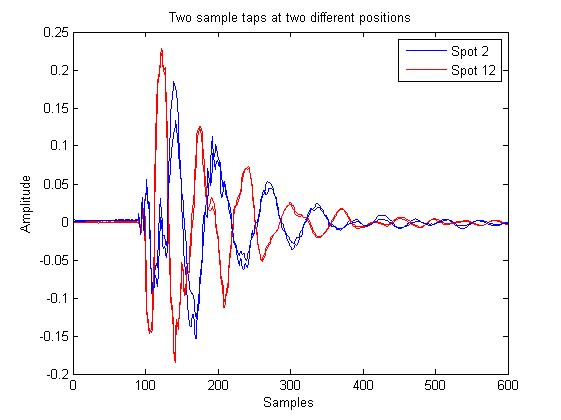
\includegraphics[width=110mm]{twotwoSampleTap}
    \caption{Two taps recorded at both spot 2 and 12 (refer to Figure~\ref{fig:phoneDisplayNum} for spot location). Sampled at 44.1 kHz.}\label{fig:twotwoSampleTap}
  \end{center}
\end{figure}

%Maybe not use this paragraph... rewrite at least.
Although Figure~\ref{fig:twotwoSampleTap} shows the scope of the variability in the pulses due to impact site, it is worth recognizing that this variability is fairly modest compared to the variability observed when comparing tapping pulses with data such as speech or even other percussive signals. It is also worth noting that some variability arises from certain environmental conditions, so the nature of the problem can be summed up as being one where certain variations are expected and others are used as the basis for classification.

\section{System}\label{sec:APRsystem}
The system developed consists of a number of different elements that crudely can be divided into hardware and software. The hardware system can be considered as a testing rig for the algorithm and is designed to facilitate a single output, black box type, approach to the classification problem, where the black box represents a unknown complex vibrational system with certain transfer characteristics. These characteristics are assumed to be reproducible or time-invariant. Figure~\ref{fig:blackBox} represents such a system, where $x^j$ can be considered some pulse on a spot $j$ known by the user, while $y$ is the output of the black box as seen by the classification algorithm oblivious to the origin of the tap $j$.

\begin{figure}[!]
\centering
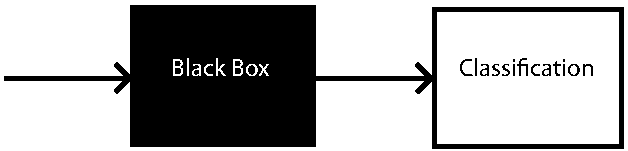
\includegraphics[width=100mm]{blackBox.pdf}
\caption{Black box representation of structural uncertainty in a tapping device.}\label{fig:blackBox}
\begin{picture}(0,0)
\put(-120,83){$x^j$}
\put(22,83){$y$}
\end{picture}
\end{figure}

Two pieces of hardware were produced to achieve these characteristics. Firstly a mobile phone implementation of the algorithm was considered and an actual mobile phone handset was acquired and modified to allow for external analogue monitoring of the internal microphone. The mobile phone chosen for this application was a Samsung SGH-M150, which can be seen in Figure~\ref{fig:phone}. This device was chosen based on its ability to be easily modified to allow for external interfacing with the microphone. Additionally a grid of $J = 12$ points was added to the screen area as reference points for tapping.

\begin{figure}[!]
\centering
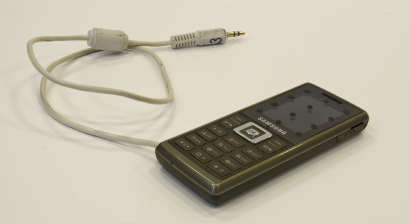
\includegraphics[width=410 px]{phone.png}
\caption{Picture of modified Samsung SGH-M150 mobile phone with 12 spot grid on display area.}\label{fig:phone}
\end{figure}

A larger application of the same black box characteristics is a simple wooden board, measuring $30.6 \times 24.3 \times 1.8$ cm (l$\times$w$\times$d), with a grid of 30 spots marked on the face of it. Attached on the back of the board, in a small cavity, is a microphone to pick up an acoustic signal from the board when tapped.  The board can be seen in Figure~\ref{fig:Pad}. The microphone used for this application is a DPA Microphone 4060 omnidirectional condenser microphone. This microphone was chosen for its excellent linear characteristics, its high sensitivity and dynamic range.

\begin{figure}[!]
\centering
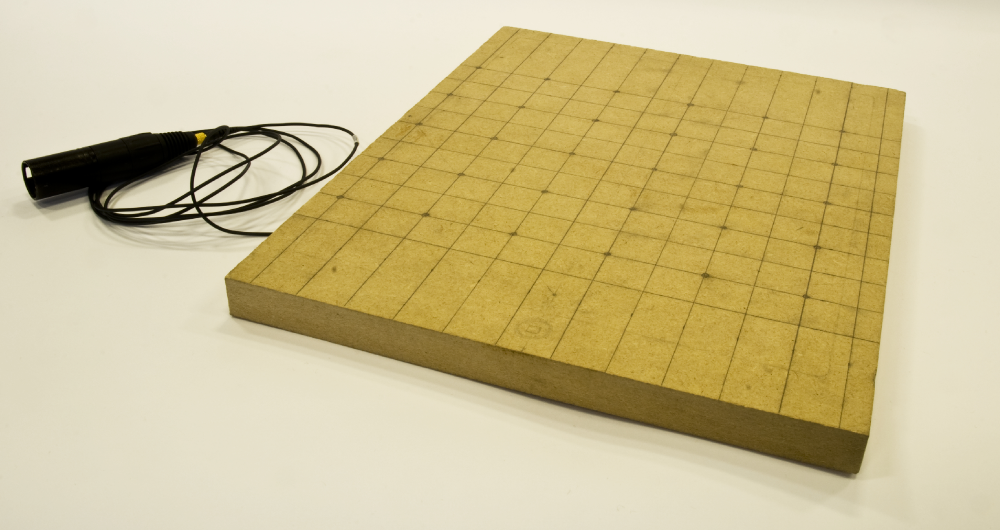
\includegraphics[width=410 px]{Pad.png}
\caption{Picture of wooden board with attached microphone to the back and 30 spot grid on the front.}\label{fig:Pad}
\end{figure}

The second part of the system is the software. Figure~\ref{fig:system} shows a simple block diagram representing the system where the bottom row is meant to represent the software system. The display on this figure represents the output from the interpolation extension to the \gls{ml} and \gls{map} methods, described later in the chapter. In this system definition, the hardware can be viewed as being the ``restricting'' factor while the software is the ``redeeming'' factor, and hence the attention is now turned to the models and algorithms of the system.

\begin{figure}[!htbp]
  \centering
    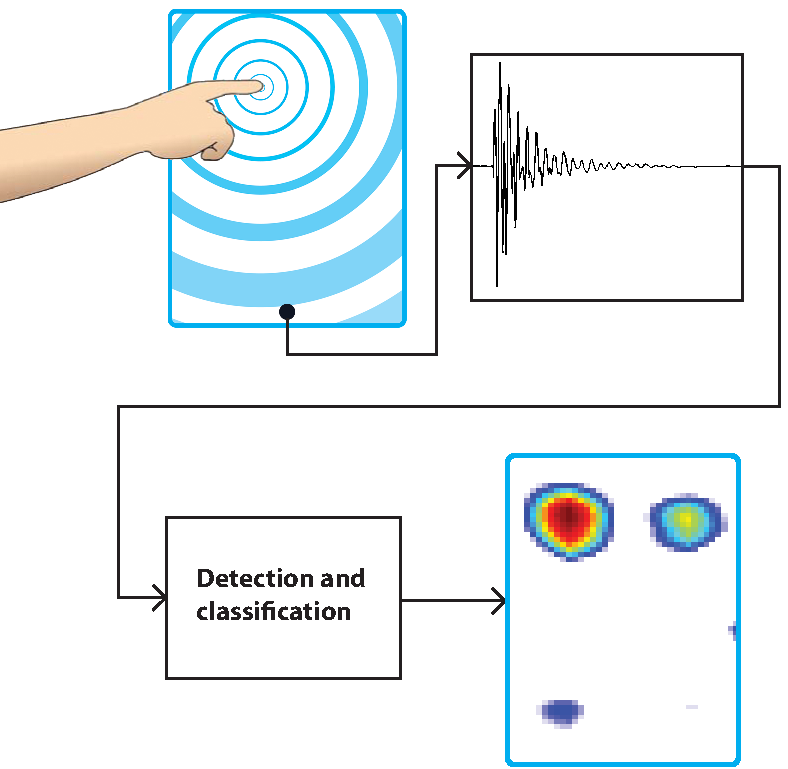
\includegraphics[width=110mm]{system.pdf}
    \caption{Block diagram of detection system. The display displays an intensity map of likelihoods superimposed on the device, as described in the extension to the \gls{ml} and \gls{map} methods.}\label{fig:system}
\begin{picture}(0,0)
\put(-136,239){Microphone}
\put(-57,179){DSP}
\put(72,204){Display}
\put(50,364){Tapping pulse}
\put(-72,243){\vector(2,1){25}}
\end{picture}
\end{figure}

\section{ML and MAP methods}
\subsection{Model and theory}
Suppose that each data reading $y = [y_0, \ldots , y_{N-1}]^T $ is modeled by the linear model

\begin{equation}\label{eq:MLmod1}
y = \theta^j t^j(n_0) + v,
\end{equation}
where $t$ is a set of $J$ templates, of length $M$, from $J$ different spots so that $t^j(n_0)$ is then the $j$th template, $j \in \{1, \ldots ,J\}$ shifted to time $n_0$ and $\theta$ is taken to be a random variable describing the scaling of the template. The prior on $\theta$ is assumed to be normal and independent across $j$.
\begin{equation}\label{eq:MLtheta}
\theta^j \sim \mathcal{N}(\mu^j_{\theta},\sigma_{\theta,j}^2),
\end{equation}

and $v$ is the independent and identically distributed (i.i.d.) Gaussian noise, modeling the background interference:

\begin{equation}\label{eq:MLnoise}
v \stackrel{i.i.d.}{\sim} \mathcal{N}(0,\sigma^2).
\end{equation}

Templates $t^j(n_0)$ for which the alignment $n_0$ and length makes them exceed the length of available data $N$, are truncated.

Henceforth the scaling factor $\theta^j$ and template $t^j(n_0)$ will be referred to respectively as $\theta$ and $t$ for simplicity.

To evaluate which, if any, of the templates are present in the data and when they are observed we need to evaluate the probability of the template number $j$ and the time shift $n_0$ given the received data $y$ which can be described as $p(j,n_0|y)$.

Using Bayes' theorem it is found that:

\begin{equation}\label{eq:MLBayes}
p(j,n_0|y) \propto p(y|j,n_0)p(j,n_0),
\end{equation}

where $p(j,n_0|y)$ is the posterior probability, $p(y|j,n_0)$ is the likelihood and $p(j,n_0)$ is the prior probability.
Take the prior probability to be:

\begin{equation}\label{eq:MLPrior}
p(j,n_0) = \frac{1}{JN},
\end{equation}
as the expression for a non-informative prior, which can be modified with time.
The likelihood can be expressed as the marginalisation of the conditional probability of the data $y$ given the scaling $\theta$, template number $j$ and the time shift $n_0$, over $\theta$, so that:

\begin{equation}\label{eq:MLmargin}
p(y|j,n_0)=\int_\theta p(y|\theta, j, n_0) p(\theta|j,n_0) d\theta,
\end{equation}

where the product of the two normal distributions $p(y|\theta, j, n_0)$ and $p(\theta|j,n_0)$, can be expressed as a third unnormalised normal distribution and a normalising constant $z$.

\begin{equation}\label{eq:MLprod1}
\mathcal{N}_y(\theta t,\sigma^2 \textbf{I})\cdot\mathcal{N}_\theta(\mu_\theta,\sigma^2_\theta) = z \times \mathcal{N}_\theta(\hat{\mu}_\theta,\hat{\sigma}^2_\theta),
\end{equation}
where $\textbf{I}$ is the appropriate $M \times M$ identity matrix and $\mathcal{N}_\theta(\hat{\mu}_\theta,\hat{\sigma}_\theta^2)$ is the third normal distribution which is the only element on the r.h.s. which is dependent on $\theta$,

\begin{equation}\label{eq:MLtheta2}
\mathcal{N}_\theta(\mu_\theta,\sigma^2_\theta) = \frac{1}{\sqrt{2 \pi \sigma_\theta^2}} \textrm{exp}\left[-\frac{\left(\theta - \mu_\theta\right)^2}{2\sigma_\theta^2}\right],
\end{equation}

and

\begin{equation}\label{eq:MLnoise2}
\mathcal{N}_y(\theta t,\sigma^2 \textbf{I}) = \frac{1}{\left(2 \pi\right)^{\frac{M}{2}\sigma}} \textrm{exp}\left[-\frac{\left(y - \theta t\right)^T\left(y - \theta t\right)}{2\sigma^2}\right].
\end{equation}

It is now possible to write the marginalisation in equation (\ref{eq:MLmargin}) as:

\begin{equation}\label{eq:MLmargin2}
p(y|j,n_0)=\int_\theta \mathcal{N}_y(\theta t,\sigma^2 \textbf{I})\cdot\mathcal{N}_\theta(\mu_\theta,\sigma^2_\theta) d\theta = z \int_\theta \mathcal{N}_\theta(\hat{\mu}_\theta,\hat{\sigma}^2_\theta) d\theta = z,
\end{equation}

since $\int_\theta \mathcal{N}_\theta(\hat{\mu}_\theta,\hat{\sigma}^2_\theta) d\theta = 1$.

To evaluate $\hat{\sigma}^2_\theta$ and $\hat{\mu}_\theta$, the l.h.s. of equation (\ref{eq:MLprod1}) must be expanded,

\begin{eqnarray}\label{eq:MLprod3}
& & \mathcal{N}_y(\theta t,\sigma^2 \textbf{I})\cdot\mathcal{N}_\theta(\mu_\theta,\sigma^2_\theta) \\\nonumber{}\\\nonumber
& & \quad = \frac{1}{\left(2\pi\right)^{\frac{M+1}{2}} \sigma \sigma_\theta} \textrm{exp}\left[-\frac{1}{2}\left(\frac{y^Ty +\theta^2t^Tt-2\theta y^T t}{\sigma^2}+\frac{\theta^2 + \mu^2_\theta-2\theta\mu_\theta}{\sigma_\theta^2}\right)\right]\\\nonumber{}\\\nonumber
& & \quad = \frac{1}{\left(2\pi\right)^{\frac{M+1}{2}} \sigma \sigma_\theta} \textrm{exp}\left[-\frac{1}{2}\left(\theta^2 \left(\frac{1}{\sigma_\theta^2}+\frac{t^T t}{\sigma^2}\right) - 2\theta\left(\frac{y^T t}{\sigma^2}+\frac{\mu_\theta}{\sigma_\theta^2}\right) + \frac{y^Ty}{\sigma^2} +\frac{\mu_\theta^2}{\sigma_\theta^2}\right)\right].
\end{eqnarray}

Expanding the r.h.s. of equation (\ref{eq:MLprod1}) gives

\begin{eqnarray}\label{eq:MLprod4}
& & z \times \mathcal{N}_\theta(\hat{\mu}_\theta,\hat{\sigma}^2_\theta) \\\nonumber{}\\\nonumber
& & \quad = \frac{z}{\sqrt{2 \pi}\hat{\sigma}_\theta}\textrm{exp}\left[-\frac{1}{2}\left(\theta^2\frac{1}{\hat{\sigma}^2_\theta} - 2\theta\frac{\hat{\mu}_\theta}{\hat{\sigma}^2_\theta} + \frac{\hat{\mu}_\theta^2}{\hat{\sigma}^2_\theta}  \right)\right]
\end{eqnarray}

By observation between equation (\ref{eq:MLprod3}) and (\ref{eq:MLprod4}) it is found that:

\begin{eqnarray}
\label{eq:MLprod5}
\hat{\sigma}^2_\theta &=& \left(\frac{t^T t}{\sigma^2} + \frac{1}{\sigma_\theta^2}\right)^{-1} \qquad \textrm{and}\\\nonumber
\hat{\mu}_\theta &=& \left(\frac{y^T t}{\sigma^2} + \frac{\mu_\theta}{\sigma^2_\theta}\right)\hat{\sigma}^2_\theta.
\end{eqnarray}

From equation (\ref{eq:MLprod1}) we have that,

\begin{equation}\label{eq:MLprod2}
z = \frac{\mathcal{N}_y(\theta t^j,\sigma^2)\cdot\mathcal{N}_\theta(\mu_\theta,\sigma^2_\theta)}{\mathcal{N}_\theta(\hat{\mu}_\theta,\hat{\sigma}^2_\theta)}
\end{equation}

and substituting in equation (\ref{eq:MLprod3}) and (\ref{eq:MLprod4}):

\begin{eqnarray}\label{eq:MLprod6}
z &=& \frac{\frac{1}{\left(2\pi\right)^{\frac{M+1}{2}} \sigma \sigma_\theta} \textrm{exp}\left[-\frac{1}{2}\left(\theta^2 \left(\frac{1}{\sigma_\theta^2}+\frac{t^T t}{\sigma^2}\right) - 2\theta\left(\frac{y^T t}{\sigma^2}+\frac{\mu_\theta}{\sigma_\theta^2}\right) + \frac{y^T y}{\sigma^2} +\frac{\mu_\theta^2}{\sigma_\theta^2}\right)\right]}{\frac{1}{\sqrt{2 \pi}\hat{\sigma}_\theta}\textrm{exp}\left[-\frac{1}{2}\left(\theta^2\frac{1}{\hat{\sigma}^2_\theta} - 2\theta\frac{\hat{\mu}_\theta}{\hat{\sigma}^2_\theta} + \frac{\hat{\mu}_\theta^2}{\hat{\sigma}^2_\theta}  \right)\right]}.
\end{eqnarray}

Substituting in values for $\hat{\sigma}^2_\theta$ and $\hat{\mu}_\theta$ from equation (\ref{eq:MLprod5}), and with a bit of rewriting, equation (\ref{eq:MLprod6}) reduces to:

\begin{equation}\label{eq:MLprod7}
z = \frac{1}{\left(2 \pi\right)^{\frac{M}{2}}\phi \sigma \sigma_\theta}\textrm{exp}\left[-\frac{1}{2}\left(\frac{y^T y}{\sigma^2}+\frac{\mu_\theta^2}{\sigma_\theta^2} - \frac{\left(\frac{y^T t}{\sigma^2}+\frac{\mu_\theta}{\sigma_\theta^2}\right)^2}{\phi}\right)\right],
\end{equation}

where $\phi = \hat{\sigma}^{-2}_\theta = \frac{t^Tt}{\sigma^2} + \frac{1}{\sigma_\theta^2}$. Remembering equation (\ref{eq:MLmargin2}) \linebreak[0]where \linebreak[0]$p(y|j,n_0) = z$, the probability of the data $y$ conditional on the model $j$ and the time shift $n_0$ is now known and can be referred to as the likelihood of the model $j$. An estimate of the model present in the data can be found by inspecting the likelihood function over the range of models. This method is called the maximum likelihood estimate or \gls{ml} estimate, and is given by:

\begin{equation}\label{eq:MLdefinition}
j_{ML} = \argmax{j} p(y|j,n_0).
\end{equation}

It is often useful to consider the log-likelihood rather than the likelihood due to machine accuracy considerations and the inherent numerical properties of the exponential function. It is worth noting that the log-likelihood and the likelihood give the same estimate since log is a monotonic transformation.

The log-likelihood is found to be:

\begin{equation}\label{eq:MLloglikelihood}
\log{p(y|j,n_0)} = -\frac{M\log{2\pi}}{2} - 0.5\log{\phi} - \log{\sigma} -\log{\sigma_\theta} - \frac{y^T y}{2\sigma^2} -\frac{\mu^2_\theta}{2\sigma^2_\theta} + \frac{\left(\frac{y^T t}{\sigma^2}-\frac{\mu_\theta}{\sigma^2_\theta}\right)^2}{2\phi},
\end{equation}

where several other constant elements can be eliminated for simplicity.

Another useful statistic to consider is the \gls{map} estimate of the model $j$. The \gls{map} estimate is given by:

\begin{equation}\label{eq:MAPdefinition}
j_{MAP} = \argmax{j} p(y|j,n_0)p(j,n_0).
\end{equation}


\section{PCA type method}\label{sec:APRpca}
While the \gls{ml} and \gls{map} methods provide a simple and reasonably effective model selection algorithm, a range of environmental factors can impact upon the recorded pulse. Figure~\ref{fig:shiftOverTemperature} shows 6 different mean templates recorded at 6 different temperatures in the range of 19.5 to 34.4 $^\textrm{o}$C.

\begin{figure}[!]
\centering
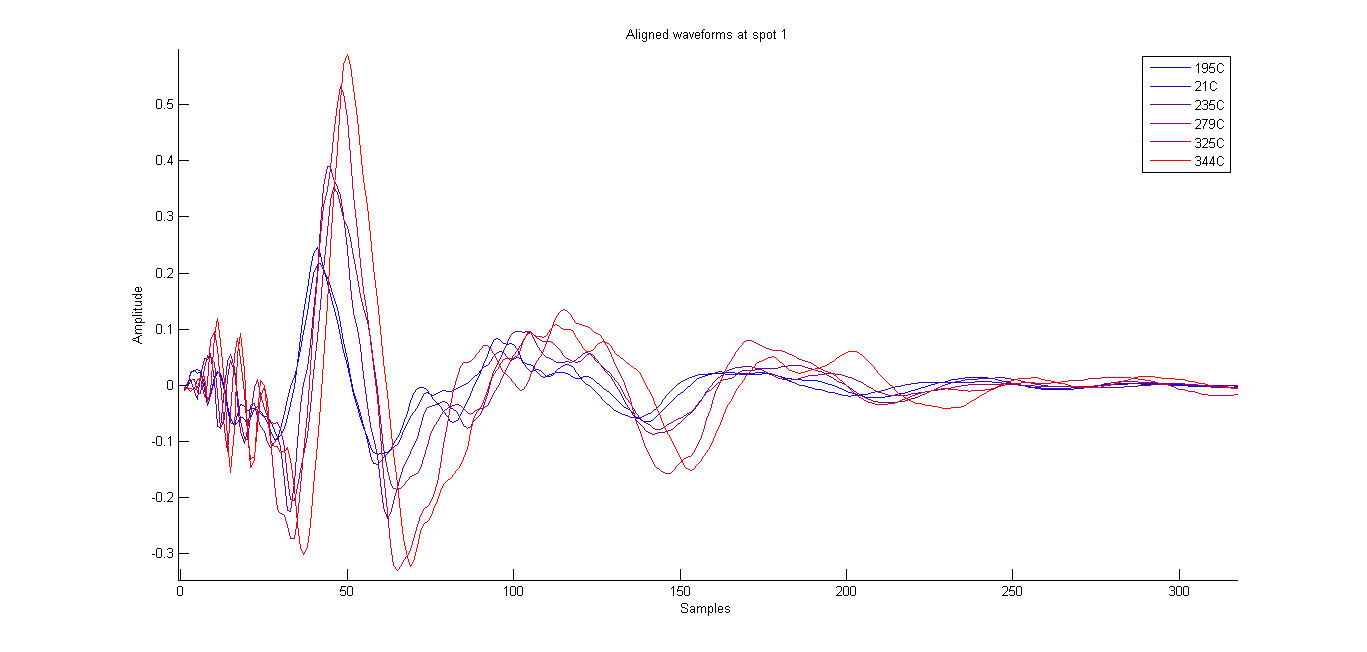
\includegraphics[width=150mm]{shiftOverTemperature.png}
\caption{6 different mean templates trained a 6 different temperatures on the same spot. Sampled at 44.1 kHz and aligned.}\label{fig:shiftOverTemperature}
\end{figure}
It appears that temperature has a dramatic effect on the mean template and therefore it seems questionable whether or not the previously described \gls{ml} and \gls{map} method would be able to cope with this level of variation. Pulse variability has also been detected when users hold the devices in different ways, have the device on a surface and tap with nails or different styluses. The \gls{pca} type method is an attempt at singling out significant components of the pulse that relate to the tapping position rather than the other factors mentioned above, and to record the variability within the significant components.

\begin{figure}[!]
\centering
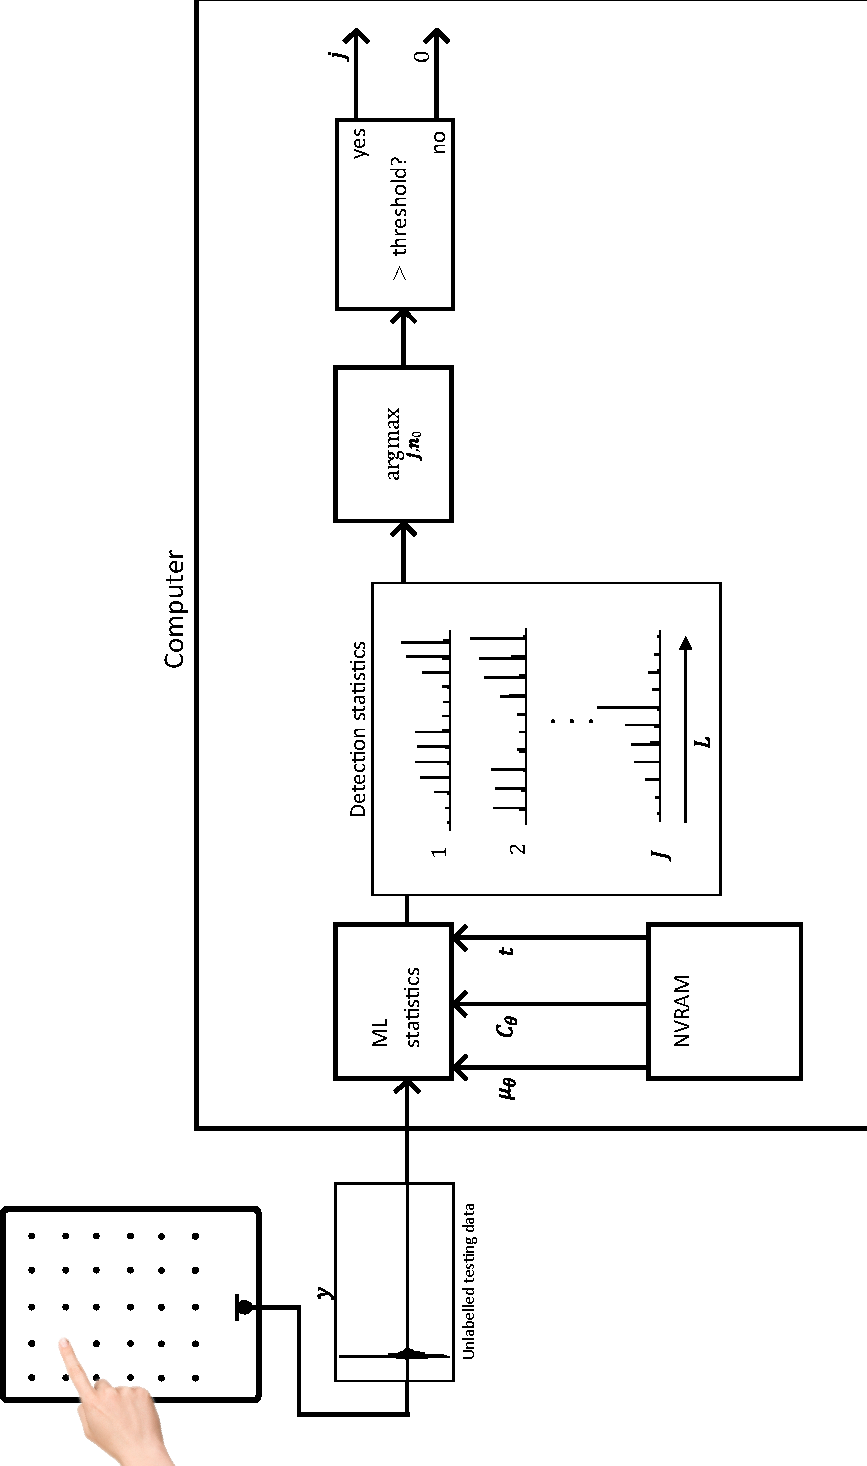
\includegraphics[width=360px]{testingSystemPlot.pdf}
\caption{Block diagram of detection/use stage of algorithm.}\label{fig:testingSystemPlot}
\end{figure}

Figure~\ref{fig:testingSystemPlot} shows a block diagram of the implementation of the use/testing stage of the algorithm. The diagram shows how a tap $y$ incident on the tapping device is picked up by the microphone on the device and transmitted to a computer. Within the computer the algorithm calculates the statistics, as outlined below, utilising data from the training stage of the algorithm. The statistics of the signal are then evaluated and the most probable class or spot is displayed to the user unless the models do not yield a sufficiently high probability, as determined by a threshold, in which case no tap will be registered.

\subsection{Model and theory}
A standard linear instantaneous model is considered where\linebreak[0] observations \linebreak[2]$y = [y_0, \ldots , y_{N-1}]^T $ are modeled as a noisy linear combination:

\begin{equation}\label{eq:mod1}
y = \sum_{i=1}^{I} \theta_i^j t_i^j(n_0) + v,
\end{equation}

where $\theta_i^j$ is the amplitude of the $j$th spot and $i$th component. $t_i^j(n_0)$ is the $j$th template, $j \in \{1, \ldots ,J\}$, for $I$ independent components where the templates are $N \times 1$ principal component vectors derived from a \gls{pca} of training data, as explained in more detail in section~\ref{sec:APRtraining}.

In this section the model has been assumed to be of zero mean $\mu^j(n_0) =0$ although this assumption could easily be avoided by adding the mean to the model as a variable to be estimated. Take $\theta_i^j$ to be a random variable, $\Theta^j = [\theta_1^j,\ldots,\theta_I^j]^T$, describing the scale of each template component $i$ where

\begin{equation}\label{eq:theta}
\Theta^j \sim \mathcal{N}(\mu_{\Theta}^j,C_{\Theta}^j),
\end{equation}

and Gaussian noise to model background interference:

\begin{equation}\label{eq:noisePCA}
v_n \stackrel{i.i.d.}{\sim} \mathcal{N}(0,\sigma^2).
\end{equation}

Considering this model in matrix notation:
\begin{equation}\label{eq:mod2PCA}
y = \textbf{t}\Theta + \textbf{v}.
\end{equation}

For simplicity the matrices $\textbf{t}^j(n_0)$ and $\Theta^j$ will from now on be referred to as simply $\textbf{t}$ and $\Theta$ respectively.
Bayes' theorem can now be used to evaluate the joint probability of $y$ and $\Theta$ as

\begin{equation}\label{eq:bayes1}
p(y,\Theta | j) = p(y|\Theta,j)p(\Theta | j).
\end{equation}

Since the goal is to evaluate the probability of each data reading $y$ given a particular position/model $j$, the dependency of $\Theta$ can be marginalized out,

\begin{eqnarray}\nonumber
p(y|j) &=& \int_\Theta p(y,\Theta|j) d\Theta \\
\label{eq:marg1} &=& \int_\Theta p(y|\Theta,j)p(\Theta|j) d\Theta.
\end{eqnarray}

Given (\ref{eq:noisePCA}) and (\ref{eq:mod2PCA}), the probability $p(y|\Theta,j)$ can be expressed as:

\begin{equation}\label{eq:probybeta}
p(y|\Theta,j) = \mathcal{N}_y(\textbf{t}\Theta,\sigma^2\textbf{I}),
\end{equation}
where $\textbf{I}$ is the identity matrix.
Now (\ref{eq:marg1}) can be written as:

\begin{equation}\label{eq:marg2}
p(y|j) = \int_\Theta \mathcal{N}_y(\textbf{t}\Theta,\sigma^2 \textbf{I})\times\mathcal{N}_\Theta(\mu_\Theta,C_\Theta) d\Theta
\end{equation}

The product of two normal distributions is another normal distribution and since this resulting normal distribution is no longer normalised a normalising constant $z$ is added:

\begin{equation}\label{eq:prod1}
\mathcal{N}_y(\textbf{t}\Theta,\sigma^2 \textbf{I})\cdot\mathcal{N}_\Theta(\mu_\Theta,C_\Theta) = z \times \mathcal{N}_\Theta(\hat{\mu}_\Theta,\hat{C}_\Theta)
\end{equation}

Since:
\begin{equation}\label{eq:marg3}
\int_\Theta \mathcal{N}_\Theta(\hat{\mu}_\Theta,\hat{C}_\Theta) d\Theta = 1,
\end{equation}
we have:
\begin{equation}\label{eq:marg4}
p(y|j) = z \times \int_\Theta \mathcal{N}_\Theta(\hat{\mu}_\Theta,\hat{C}_\Theta) d\Theta = z.
\end{equation}

To evaluate $z$, the l.h.s. of equation (\ref{eq:prod1}) is expanded
{\setlength\arraycolsep{2pt}
\begin{eqnarray}
\label{eq:prod2} & & \mathcal{N}_y(\textbf{t}\Theta,\sigma^2 \textbf{I})\times\mathcal{N}_\Theta(\mu_\Theta,C_\Theta) = \\\nonumber
& & \qquad \frac{1}{(2\pi)^{\frac{N}{2}} |\sigma^2\textbf{I}|^{\frac{1}{2}}} \textrm{exp}\left[-\frac{1}{2}(y - \textbf{t}\Theta)^T(\sigma^2 \textbf{I})^{-1}(y - \textbf{t}\Theta)\right] \times {} \\\nonumber
& & \qquad \frac{1}{(2\pi)^{\frac{N}{2}}|C_\Theta|^{\frac{1}{2}}} \textrm{exp}\left[-\frac{1}{2}(\Theta - \mu_\Theta)^TC_\Theta^{-1}(\Theta - \mu_\Theta)\right] \\\nonumber
& & \quad= \frac{1}{(2\pi)^N |\sigma^2\textbf{I}|^{\frac{1}{2}} |C_\Theta|^{\frac{1}{2}}} \textrm{exp}\bigg[-\frac{\textbf{I}}{2\sigma^2}\left(y^Ty+\Theta^T\textbf{t}^T\textbf{t}\Theta - 2 \Theta^T\textbf{t}y\right) - {} \\\nonumber
& & \qquad \frac{1}{2C_\Theta} \left(\Theta^T\Theta + \mu_\Theta^T\mu_\Theta - 2 \Theta^T\mu_\Theta\right) \bigg] \\\nonumber
& & \quad = \frac{1}{(2\pi)^N |\sigma^2\textbf{I}|^{\frac{1}{2}} |C_\Theta|^{\frac{1}{2}}} \textrm{exp}\Bigg[-\frac{1}{2}\Bigg(\Theta^T\left(\frac{\textbf{t}^T\textbf{t}}{\sigma^2} + C_\Theta^{-1}\right)\Theta - 2 \Theta^T\left(\frac{\textbf{t}y}{\sigma^2} + \frac{\mu_\Theta}{C_\Theta}\right) + {}\\\nonumber
& & \qquad \mu_\Theta^TC_\Theta^{-1}\mu_\Theta + \frac{y^Ty}{\sigma^2}\Bigg)\Bigg].
\end{eqnarray}}
The r.h.s. of equation (\ref{eq:prod1}) is also expanded,

{\setlength\arraycolsep{2pt}
\begin{eqnarray}
\label{eq:prod3} & & z \times \mathcal{N}_\Theta(\hat{C}_\Theta,\hat{\mu}_\Theta) \\\nonumber
& & \quad = z\frac{1}{(2\pi)^{\frac{N}{2}} |\hat{C}_\Theta|^{\frac{1}{2}}} \textrm{exp}\left[-\frac{1}{2}\left(\Theta - \hat{\mu}_\Theta\right)^T\hat{C}_\Theta^{-1}\left(\Theta - \hat{\mu}_\Theta\right)\right] \\\nonumber
& & \quad = z\frac{1}{(2\pi)^{\frac{N}{2}} |\hat{C}_\Theta|^{\frac{1}{2}}} \textrm{exp}\left[-\frac{1}{2}\left(\Theta^T\hat{C}_\Theta^{-1}\Theta + \hat{\mu}_\Theta^T\hat{C}_\Theta^{-1}\hat{\mu}_\Theta - 2\Theta^T\hat{C}_\Theta^{-1}\hat{\mu}_\Theta\right)\right],
\end{eqnarray}}
and by inspection and comparison between equation (\ref{eq:prod2}) and (\ref{eq:prod3}) it is found that:

\begin{eqnarray}
\label{eq:prod4}
\hat{C}_\Theta &=& \left(\frac{\textbf{t}^T\textbf{t}}{\sigma^2} + C_\Theta^{-1}\right)^{-1} \qquad \textrm{and}\\\nonumber
\hat{\mu}_\Theta &=& \left(\frac{\textbf{t}^Ty}{\sigma^2} + \frac{\mu_\Theta}{C_\Theta}\right)\hat{C}_\Theta.
\end{eqnarray}

Equation (\ref{eq:prod2}) and (\ref{eq:prod3}) are equated and the normalizing constant $z$ is isolated.

{\setlength\arraycolsep{2pt}
\begin{eqnarray}\label{eq:z1}
z &=& \frac{(2\pi)^{\frac{N}{2}}\left|\hat{C}_\Theta\right|^{\frac{1}{2}} }{(2\pi)^n |\sigma^2\textbf{I}|^{\frac{1}{2}} |C_\Theta|^{\frac{1}{2}}} \times {}\\\nonumber
& &\frac{\textrm{exp}\Bigg[-\frac{1}{2}\Bigg(\Theta^T\left(\frac{\textbf{t}^T\textbf{t}}{\sigma^2} + C_\Theta^{-1}\right)\Theta - 2 \Theta^T\left(\frac{\textbf{t}y}{\sigma^2} + \frac{\mu_\Theta}{C_\Theta}\right) + \mu_\Theta^TC_\Theta^{-1}\mu_\Theta + \frac{y^Ty}{\sigma^2}\Bigg)\Bigg]}{\textrm{exp}\left[-\frac{1}{2}\left(\Theta^T\hat{C}_\Theta^{-1}\Theta - 2\Theta^T\hat{C}_\Theta^{-1}\hat{\mu}_\Theta + \hat{\mu}_\Theta^T\hat{C}_\Theta^{-1}\hat{\mu}_\Theta \right)\right]}.
\end{eqnarray}}
Substituting $\hat{C}_\Theta$ from equation~(\ref{eq:prod4}) and doing some simplification, gives:
{\setlength\arraycolsep{2pt}
\begin{eqnarray}\label{eq:z2}
z &=& \frac{\left|\frac{\textbf{t}^T\textbf{t}}{\sigma^2} + C_\Theta^{-1}\right|^{-\frac{1}{2}}}{(2\pi)^{\frac{n}{2}} |\sigma^2\textbf{I}|^{\frac{1}{2}} |C_\Theta|^{\frac{1}{2}}} \times {}\\\nonumber
& &\frac{\textrm{exp}\Bigg[-\frac{1}{2}\Bigg(\Theta^T\left(\frac{\textbf{t}^T\textbf{t}}{\sigma^2} + C_\Theta^{-1}\right)\Theta - 2 \Theta^T\left(\frac{\textbf{t}y}{\sigma^2} + \frac{\mu_\Theta}{C_\Theta}\right) +  \mu_\Theta^TC_\Theta^{-1}\mu_\Theta + \frac{y^Ty}{\sigma^2}\Bigg)\Bigg]}{\textrm{exp}\left[-\frac{1}{2}\left(\Theta^T \left(\frac{\textbf{t}^T\textbf{t}}{\sigma^2} + C_\Theta^{-1}\right)\Theta  - 2\Theta^T\left(\frac{\textbf{t}^T\textbf{t}}{\sigma^2} + C_\Theta^{-1}\right)\hat{\mu}_\Theta  + \hat{\mu}_\Theta^T\left(\frac{\textbf{t}^T\textbf{t}}{\sigma^2} + C_\Theta^{-1}\right)\hat{\mu}_\Theta \right)\right]}
\end{eqnarray}}
Substituting $\hat{\mu}_\Theta$ from equation~(\ref{eq:prod4}) and doing some simplification, gives:
{\setlength\arraycolsep{2pt}
\begin{eqnarray}\label{eq:z25}
z &=& \frac{1}{(2\pi)^{\frac{n}{2}} |\textbf{t}^T\textbf{t}+\sigma^2C_\Theta^{-1}|^{\frac{1}{2}} |C_\Theta|^{\frac{1}{2}}} \times {}\\\nonumber
& &\frac{\textrm{exp}\Bigg[-\frac{1}{2}\Bigg(- 2 \Theta^T\left(\frac{\textbf{t}y}{\sigma^2} + \frac{\mu_\Theta}{C_\Theta}\right) +  \mu_\Theta^TC_\Theta^{-1}\mu_\Theta + \frac{y^Ty}{\sigma^2}\Bigg)\Bigg]}{\textrm{exp}\left[-\frac{1}{2}\left(- 2\Theta^T\left(\frac{\textbf{t}^Ty}{\sigma^2} + \frac{\mu_\Theta}{C_\Theta}\right)  + \left(\left(\frac{\textbf{t}^T\textbf{t}}{\sigma^2} + C_\Theta^{-1}\right)^T\right)^{-1}\left(\frac{\textbf{t}^Ty}{\sigma^2} + \frac{\mu_\Theta}{C_\Theta}\right)^T\left(\frac{\textbf{t}^Ty}{\sigma^2} + \frac{\mu_\Theta}{C_\Theta}\right) \right)\right]}\\\nonumber{}\\\nonumber
&=& \frac{1}{(2\pi)^{\frac{n}{2}} |\Phi|^{\frac{1}{2}} |C_\Theta|^{\frac{1}{2}}}\times \frac{\textrm{exp}\left[-\frac{1}{2\sigma^2}\left(\sigma^2\mu_\Theta^TC_\Theta^{-1}\mu_\Theta + y^Ty\right)\right]}{\textrm{exp}\left[-\frac{1}{2\sigma^2}\left(\left(\Phi^T\right)^{-1}\Lambda^T\Lambda \right)\right]}\\\nonumber{}\\\nonumber
&=& \frac{1}{(2\pi)^{\frac{n}{2}} |\Phi|^{\frac{1}{2}}|C_\Theta|^{\frac{1}{2}}} \textrm{exp}\left[-\frac{1}{2\sigma^2}\left(\sigma^2\mu_\Theta^TC_\Theta^{-1}\mu_\Theta + y^Ty- \left(\Phi^T\right)^{-1}\Lambda^T\Lambda\right)\right],
\end{eqnarray}}
where:
\begin{eqnarray}
\label{eq:z3}
\Phi &=& \textbf{t}^T\textbf{t} + \sigma^2C_\Theta^{-1} \qquad \textrm{and}\\\nonumber
\Lambda &=& \textbf{t}^Ty + \sigma^2\mu_\Theta C_\Theta^{-1}.
\end{eqnarray}

As with the previous method, the log-likelihood is calculated

\begin{equation}\begin{split}\label{eq:loglikeli}
\log{p(y|j)} = &- \frac{n}{2}\log{2 \pi}- \frac{1}{2}\log{|\Phi|} - \frac{1}{2}\log{|C_\Theta|} \\
&- \frac{1}{2\sigma^2}\left(\sigma^2\mu_\Theta^TC_\Theta^{-1}\mu_\Theta + y^Ty- \left(\Phi^T\right)^{-1}\Lambda^T\Lambda\right),
\end{split}\end{equation}

and maximised over the $J$ different templates, similar to equation~(\ref{eq:MLdefinition}).

\section{Amplitude variable PCA model}\label{sec:KamplitudeModel}

To account for linear scaling of the signal $x$, a modified \gls{pca} model is constructed. While the $\theta$ parameter of the \gls{pca} approach assumes that each pulse is a combination of a set of components observed during training, the strength of impact on the surface will translate into an increased amplitude of the pulse waveform. The aim of the variable amplitude model is to separate out this scale as a random variable $K$. In the basic \gls{pca} model the pulse amplitudes were represented in the $\theta$ parameter and in this model the amplitudes will be represented as $K$ and then subsequently normalized. 

Recalling the standard multi-variate \gls{pca} based approach with mean $\mu$ zero (see equation \ref{eq:mod1}), we had

\begin{equation}\label{eq:K_PCAmodel}
y = \sum^I_{i=1} \theta^j_i t^j_i(n_0) + v.
\end{equation}

For $K$ a vector of scalar amplitudes for the combined instantaneous linear combination, we can write,

\begin{equation}\label{eq:Kmodel}
y = K^j \sum^I_{i=1} \theta^j_i t^j_i(n_0) + v.
\end{equation}

Here $K^j$ is the scaling amplitude for the $j$th template.

Considering previously equation~\ref{eq:probybeta}, we can now model the signal $y$ as:

\begin{equation}\label{eq:GP2}
    p(y|j,n_0,K) = \mathcal{N}_y(K^j \Theta^j \textbf{t}^j(n_0) , \sigma^2),
\end{equation}

where $K_j$ is a random variable describing the linear scaling of the model.

In equation~\ref{eq:MLmargin} the continuous component scaling factor $\theta$ was marginalised out to give $p(y|j,n_0)$. In much the same way, the likelihood can be estimated by evaluation of the joint probability of the data $y$ given a discrete scaling $K$, template number $j$ and the time shift $n_0$, over $K$.

For $K$, $p(K)$ is now considered to be a discretely sampled distribution such that

\begin{equation}\label{eq:pkldefine}
Pr\left\{K = k_l\right\} = p_{K,l},
\end{equation}

for the $l = 1:L$ samples of $p(K)$.

The sampling of $p(K)$ can now be expressed as
\begin{equation}\label{eq:sampledK}
p(K|j) = \sum_{l=1}^L p^j_{K,l} \delta \left(K - k_l\right),
\end{equation}

and the signal $y$ can now be modeled as

\begin{eqnarray}\label{eq:MLmarginK}
p(y|j,n_0) &=& \int \sum_{l=1}^L p(y|j, n_0, K=k_l) p^j_{K,l} \delta \left(K - k_l\right) dK\\
&=& \sum_{l=1}^L p(y|j, n_0, K=k_l) p^j_{K,l}.
\end{eqnarray}

The distribution of $p(K|j)$ could be estimated as a discrete point-mass \linebreak[0](positive-valued) inverse-gamma distribution or simply sampled at a training stage for each class $j$. In this case $p(K|j)$ is assumed to be discrete and equation~\ref{eq:MLmarginK} is a finite sum of weighted Gaussian terms. In the continuous cases the integral could be computed using Monte Carlo integration approximated using discrete summation.

Proceeding with the steps from equation~\ref{eq:marg2} - \ref{eq:z25} (the full derivations are available in Appendix~\ref{ap:AppDeriv}, the log-likelihood is calculated

\begin{equation}\label{eq:loglikeliK}\begin{split}
\log{p(y|j,n_0,\theta,K)} = &- \frac{n}{2}\log{2 \pi}- \frac{1}{2}\log{|\Phi|} - \frac{1}{2}\log{|C_\Theta|} \\
& -\frac{1}{2\sigma^2}\left(\sigma^2\mu_\Theta^TC_\Theta^{-1}\mu_\Theta + y^Ty- \left(\Phi^T\right)^{-1}\Lambda^T\Lambda\right),
\end{split}\end{equation}

where
\begin{eqnarray}
\label{eq:z3K}
\Phi &=& K^2 \textbf{t}^T\textbf{t} + \sigma^2C_\Theta^{-1} \qquad \textrm{and}\\\nonumber
\Lambda &=& K \textbf{t}^Ty + \sigma^2\mu_\Theta C_\Theta^{-1}.
\end{eqnarray}

\section{Training}\label{sec:APRtraining}
In order to be able to deploy the above mentioned models, the templates needed in the models must be created. The term ``training'' is here used to refer to the process of creating the matrices $t$ and $t^j_i(n_0)$ containing the $J$ models and $I$ components, the covariance matrix $C^j_\Theta$ and the mean $\mu^j_\Theta$.

To train a template for a spot, a large quantity of tapping data is recorded from the device and stored. This tapping data is labeled, that is, the spot which was tapped to create the tapping pulse is known and the tapping data is divided into separate streams depending on this label. To pick out the individual taps from the audio stream, a representative tap is manually chosen from each stream and used as the coefficients in a correlation detector, the results of which are used to determine the alignment of the individual taps in the audio stream. A correlation detector, in this context, refers to a matched filter with a sample representative pulse used as the filter parameters with the output thresholded in some way. Figure~\ref{fig:correlationDetect} shows a short audio stream of taps where the red dots indicate detected taps.

\begin{figure}[!]
\centering
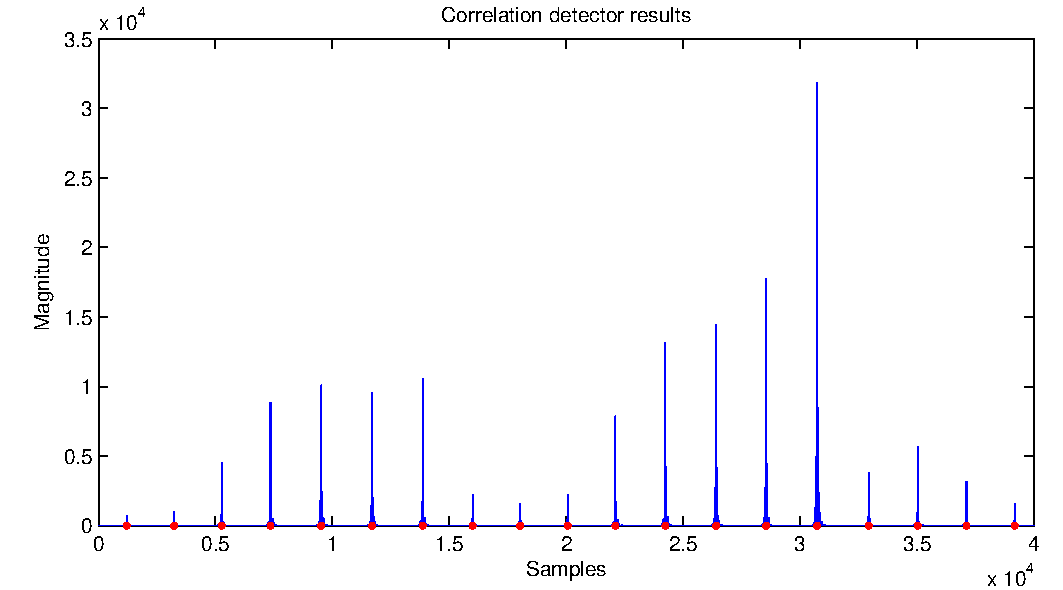
\includegraphics[width=150mm]{correlationDetect.pdf}
\caption{Output of correlation detection code. The plot shows the output of the matched filter using a manually picked pulse as a template and the red dots indicate detected taps via a simple thresholding.}\label{fig:correlationDetect}
\end{figure}

With all the taps in the audio stream detected it is now possible to align them for further processing.

\begin{figure}[!]
\centering
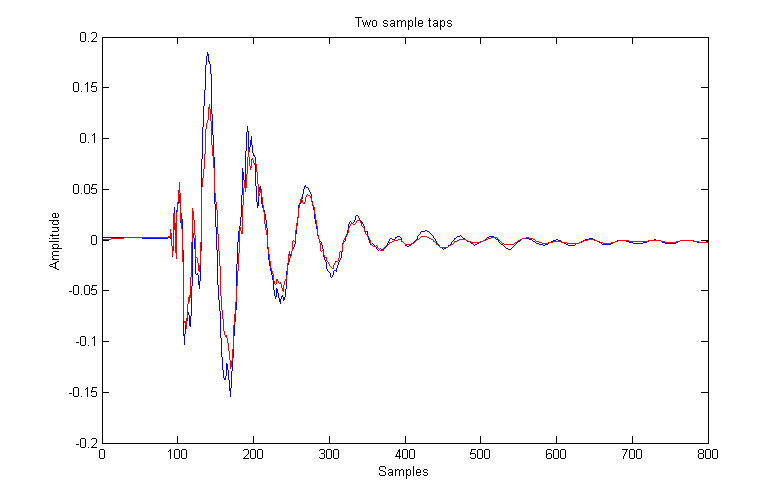
\includegraphics[width=110mm]{twoSampleTaps.png}
\caption{Two taps recorded at the same spot immediately after each other. Sampled at 44.1 kHz.}\label{fig:twoSampleTaps}
\end{figure}

Figure~\ref{fig:twoSampleTaps} shows a modest example of the variability that exists when tapping an object in seemingly the exact same manner. This variability is partly due to noise but bigger variations in the waveform are more likely caused by minute variations in tapping position, intensity and method. In an attempt to obtain a 1 dimensional model that represents a diverse selection of taps at the same spot for the \gls{ml} and \gls{map} method, the model is constructed as a mean of an ensemble of taps at this position. The mean template is manually trimmed to minimise data size and avoid excessive data that carries no useful information about the template. Figure~\ref{fig:alignedAndMean} shows a diverse set of aligned taps at a single point in blue and the corresponding mean in red.

\begin{figure}[!]
\centering
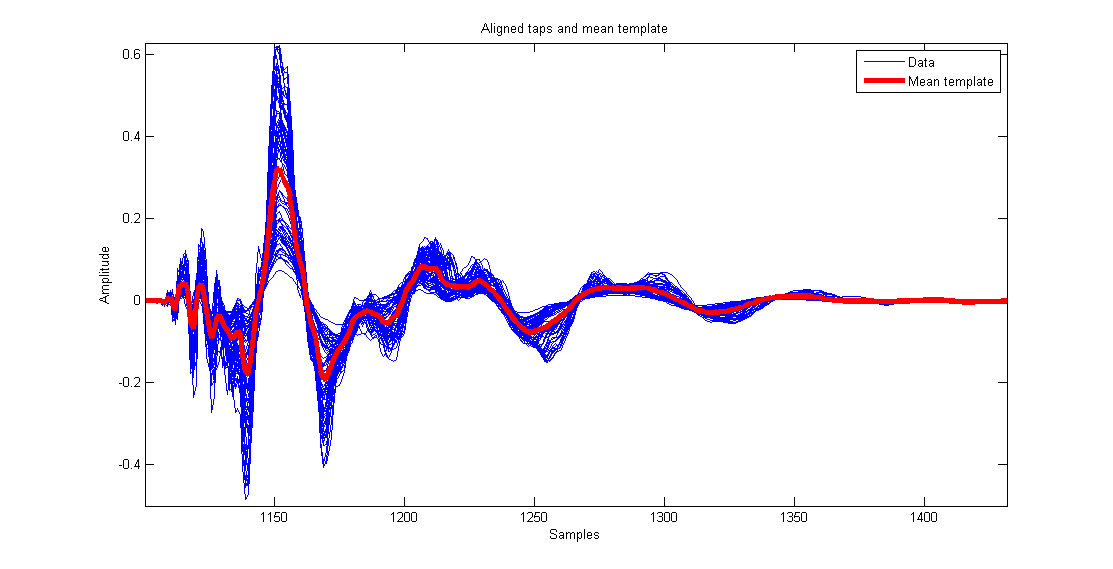
\includegraphics[width=150mm]{alignedAndMean.png}
\caption{Aligned taps with corresponding mean template superimposed on top. Sampled at 44.1 kHz.}\label{fig:alignedAndMean}
\end{figure}

Due to the nature of this algorithm it is essential that it can be executed rapidly and in real time. To accomplish a rapid execution, sub-calculations, independent of $y$, from equation (\ref{eq:MLloglikelihood}) have been pre-computed.

The \gls{pca} type method requires a different type of template. Here the template is derived via a \gls{pca} of the covariance matrix derived from the aligned tapping data as described above.

First the mean and the covariance matrices for each spot $j$ are calculated:

\begin{eqnarray}\nonumber
\mu^j &=& \frac{1}{N^j} \sum_k x^j_k \\\label{eq:PCAcovariance}
C^j &=& \frac{1}{N^j}\sum_k \left(x^j_k - \mu^j\right)\left(x^j_k - \mu^j\right)^T,
\end{eqnarray}
where $x^j_k$ is the $k$th segment of the tapping stream containing a tap on the $j$th spot and $N^j$ is the sample length of the $j$th template. The eigenvalues and the eigenvectors of the covariance matrices $C^j$ are then computed, and the required number of components $q$ (eigenvectors) are chosen based on the corresponding descending values of the eigenvalue. Figure~\ref{fig:eigenvalues} shows an example of a descending order of eigenvalues from an eigenvalue decomposition of the covariance matrix $C^j$.

\begin{figure}[!]
\centering
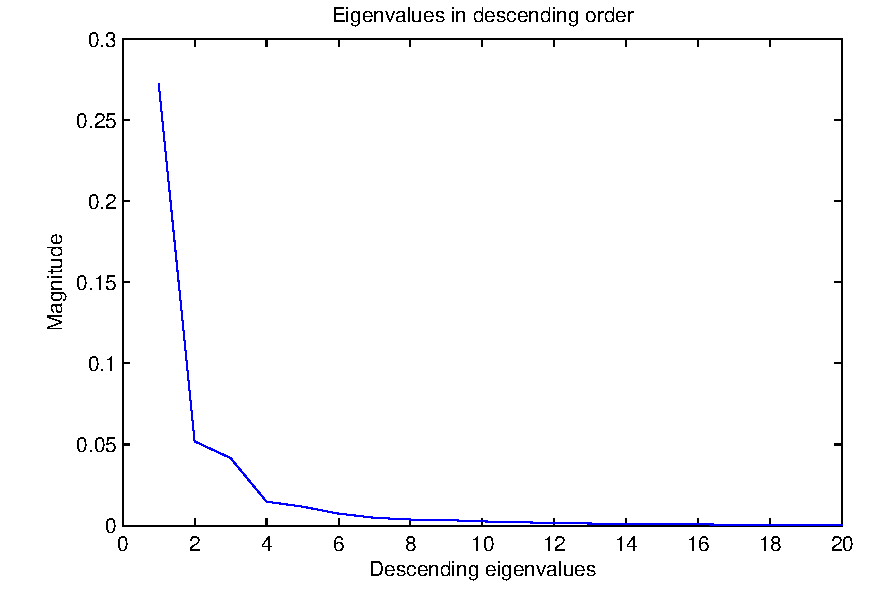
\includegraphics[width=120mm]{eigenvalues.pdf}
\caption{Descending eigenvalues from a eigenvalue decomposition of a covariance matrix $C^j$.}\label{fig:eigenvalues}
\end{figure}

As with the previous method, it is also possible to allocate sub-calculations independent of $y$ from equation~(\ref{eq:z2}) to the training stage to avoid heavy calculations during runtime. In addition, $\mu_\Theta$ is also defined during the training stage.

Figure~\ref{fig:trainingsytemRotate} shows a block diagram of the implementation of the training algorithm. The training data $x^j$ is acquired by the user tapping multiple times on a specific spot $j$. The $N$ taps in this data stream $x^j$ are then detected and aligned with each other as an ensemble in a matrix. Figure~\ref{fig:trainingsytemRotate} shows this as $\textbf{x}^j =  [ x_1^j, x_2^j, \ldots , x_N^j ] $ and as the $N$ taps superimposed on each other in the little plot. From the ensemble the mean $\mu^j$ and the covariance matrix $C^j$ are computed, and from the covariance matrix $C^j$ the eigenvalues and eigenvectors are derived. The $q$ largest eigenvalues are selected and the corresponding eigenvectors are stored as the templates $t^j = [\alpha^j_1,\alpha^j_2,\ldots,\alpha^j_q] $ while the eigenvalues are stored as $C_\Theta^j = diag\{\lambda_1^j,\lambda_2^j,\ldots,\lambda_q^j \}$.

\begin{figure}[!]
\centering
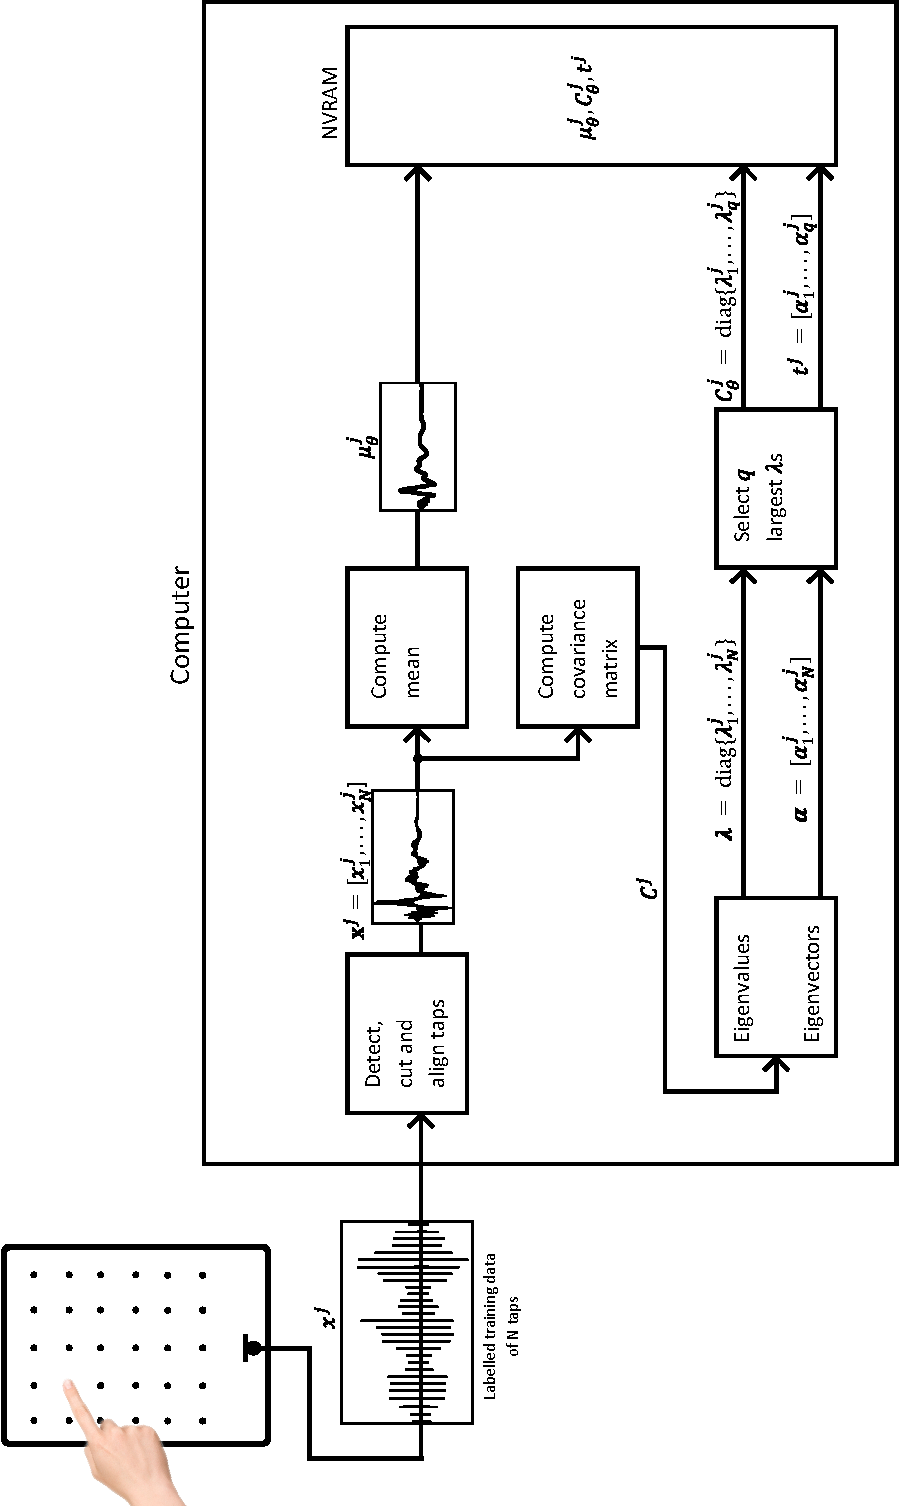
\includegraphics[width=360px]{trainingsytemRotate.pdf}
\caption{Block diagram of training stage of algorithm.}\label{fig:trainingsytemRotate}
\end{figure}

\subsection{Amplitude variable PCA model}

In addition to the parameters required for the standard \gls{pca} model, the amplitude variable model requires information about the scaling parameter $K$. Here we propose to sample $K^j = [K^j_{l=1}, \ldots , K^j_{l=L}]$, from the aligned training pulses recorded. Figure~\ref{fig:amplitudeProbMass.pdf} shows an example of the sampled probability mass functions used for three different models $j$. The sampling is done from a kernel smoothed distribution of amplitudes of the ensemble of pulses recorded. While $K^j$ is a discrete scaling vector for each model $j$ Figure~\ref{fig:amplitudeProbMass.pdf} shows continuous smoothed functions to better illustrate some of the variety in the models and to be able to plot them together. Each scaling vector $K^j$ comprises $L=100$ scales.

\begin{figure}
\centering
  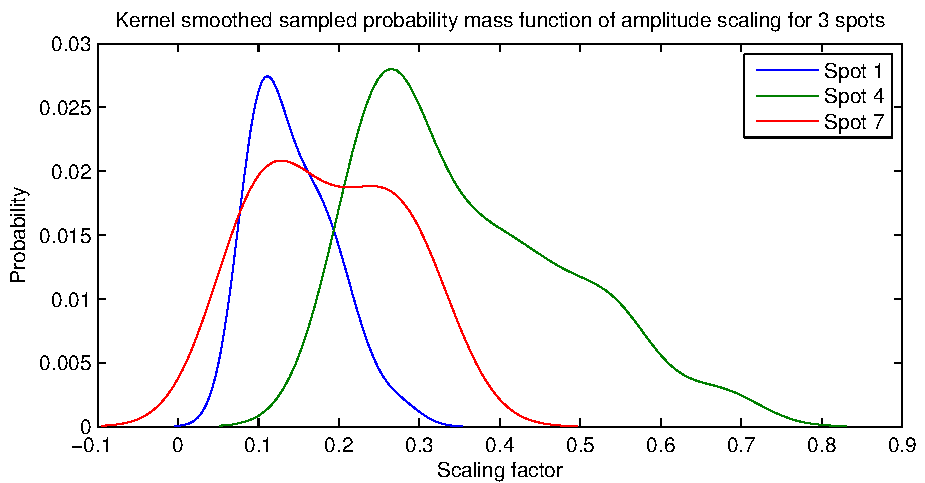
\includegraphics[width=110mm]{amplitudeProbMass.pdf}\\
  \caption{Kernel smoothed discrete probability mass function of 3 different spots for microphone 1.}\label{fig:amplitudeProbMass.pdf}
\end{figure}

\subsection{Sparse training extension}\label{sec:APRspareTraining}
The methods outlined above require labeled training data for each model in the classifier. Since it is entirely manageable to obtain this data for low resolution implementation of the pulse recognition system, obtaining this data on a larger device with a greater resolution can become cumbersome and time consuming. This extension of the standard training method for the \gls{ml} and \gls{map} methods enables detection of points outside the training grid at a scalable resolution.

To achieve this extended resolution, the algorithm creates a linear interpolation between neighboring templates. The assumption is that the acoustic pulses vary relatively linearly between the two templates and hence it may be possible to estimate any template in between the two. Since the mobile phone, used for the previous implementation, undoubtedly is a very complicated vibrational system it was hypothesised that the solid wooden board might provide a more predictable vibrational system and hence a better implementation platform for the interpolation algorithm.

For a number of tapping spots evenly distributed on a line, the interpolated template $t$ at position $x$ along the line on the board can be interpolated by

\begin{equation}\label{eq:interp}
t = t_0 + \left(x - x_0\right) \frac{t_{1} - t^j}{x_1 - x_0},
\end{equation}

where $t_0$ and $t_1$ are the templates at the positions $x_0$ and $x_1$ respectively and \linebreak[0]$x_0 < x < x_1$.

An example of a section of the waveforms resulting from this interpolation can be seen in Figure~\ref{fig:InterpData}. Here the thick lines represent the templates computed from data while the thin lines are interpolated templates. The linearly varying color, between red and black of the thin lines, shows the relative distance of the template position $x$ in this example.

\begin{figure}[!]
\centering
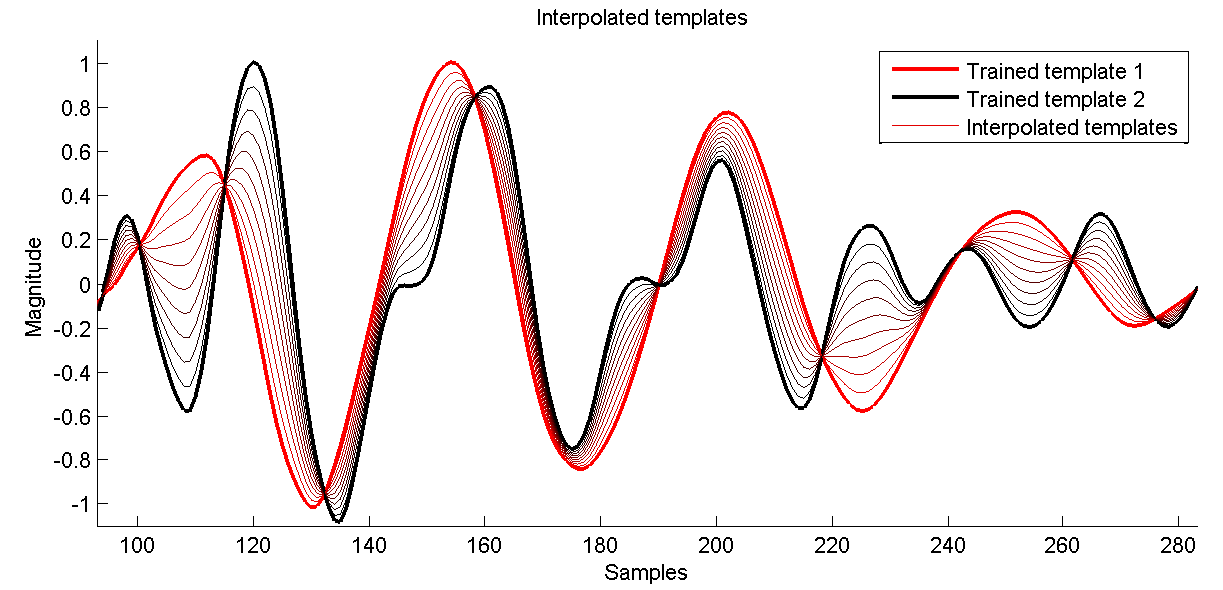
\includegraphics[width=360px]{InterpData.pdf}
\caption{Example of section of a interpolated waveforms using linear interpolation.}\label{fig:InterpData}
\end{figure}

To achieve a full 2D grid of interpolated templates amongst templates derived from data, requires a second round of interpolation in the second dimension for each column.

While the assumption of linearly changing pulses might be valid, it is still necessary to align the neighboring templates accurately. Aligning taps accurately has proven difficult with the correlation method due to the change in the pulses over the surface of the board. To provide a more accurate alignment method a second microphone was attached to the stylus while tapping to provide a consistent reference tap. The idea was that this consistent tap should provide exact alignment between all the taps. Figure~\ref{fig:templatesAligned} shows the result of this alignment.

\begin{figure}[!]
\centering
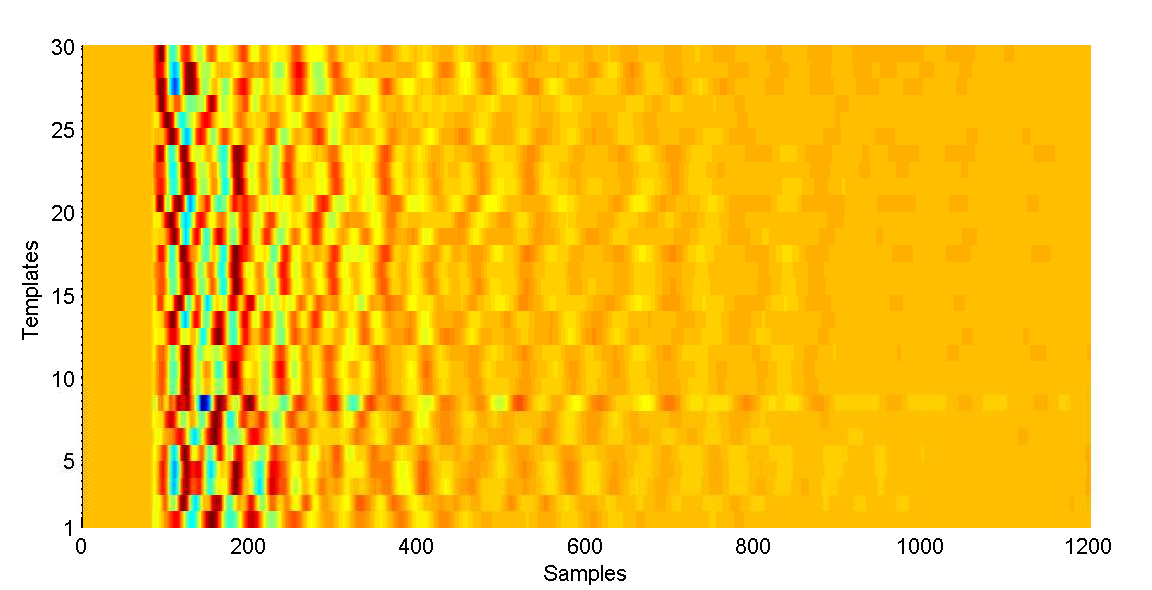
\includegraphics[width=380px]{templatesAligned.pdf}
\caption{30 templates from wooden board aligned. Seen from above.}\label{fig:templatesAligned}
\end{figure}

The benefit of a representation like Figure~\ref{fig:templatesAligned} is that it shows the wooden board is laid out in a grid of 6 by 5 spots, spot numbering starting in top left corner and following reading direction, which allows for assessment of alignment row by row.

The standard 6 by 5 spot resolution on the wooden board can be expanded to 51 by 41 spots simply by interpolating 9 templates between each trained spot row-wise and then doing the same for all 41 columns. The running of the detection algorithm will proceed as before although at a substantially slower rate.

\section{Methods}
\subsection{Performance and comparison of ML, MAP and PCA methods}
To test the algorithms, two sets of data are needed; a training set $D^1$ and a testing set $D^2$. The training set is used in the training stage of the algorithm, as mentioned above, and the testing data is essentially the data that the algorithm attempts to model and classify. In an attempt to evaluate the algorithms' robustness to variations, two different sets of training and testing data were used. One set was recorded using a stylus to tap on the device, $D^1_S$ and $D^2_S$, and the second set was tapped using a finger nail, $D^1_N$ and $D^2_N$. Although it might be informative to use the same data for the training and testing stage, in this test the two sets were independently recorded, in identical conditions, which means that there in total are 4 data sets $D^1_S$, $D^2_S$, $D^1_N$ and $D^2_N$, which will be used to test the algorithms in various combinations giving a picture of the performance of the algorithms. Figure~\ref{fig:tapSN} shows the tapping of the surface of the device with a stylus and with a fingernail.

\begin{figure}[!]
\centering
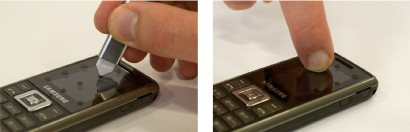
\includegraphics[width=410 px]{tapSN.png}
\caption{To the left is an example of a tap with the stylus and to the right a tap with a fingernail.}\label{fig:tapSN}
\end{figure}

\begin{figure}[!]
\centering
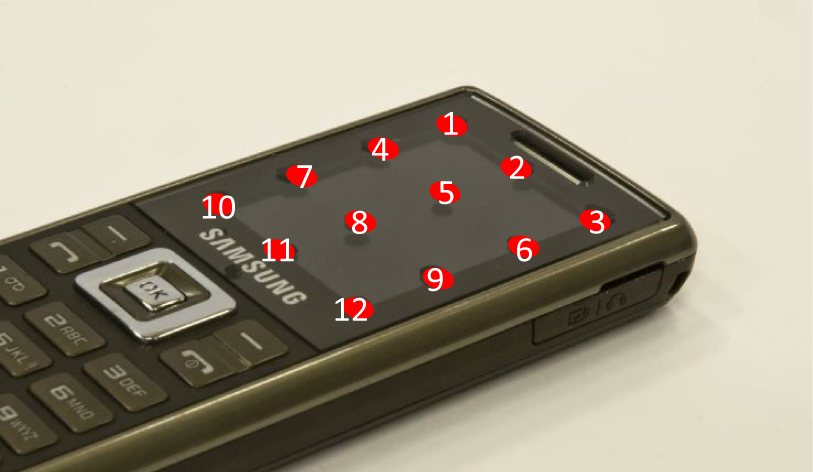
\includegraphics[width=300 px]{phoneDisplayNum.png}
\caption{Phone with spot location and numbers.}\label{fig:phoneDisplayNum}
\end{figure}

Figure~\ref{fig:phoneDisplayNum} shows the 12 spots and their location on the front of the phone used in this chapter.

Each set of training data contains approximately 70 taps at each spot on the device totalling approximately $70 \times 12 = 840$ taps tapped with varying force. To estimate the performance of the algorithm given certain criteria there are 3 outcomes of a test. The tap may be correctly classified, misclassified (classified as any of the 11 other spots) or it may avoid detection entirely and hence be classified as a missed detection $j=0$. The ratio of these 3 outcomes may vary with a large number of parameters within the algorithm such as various thresholds for detection or classification, template length, filtering or number of principal components used under training, so the performance of the algorithm will always be presented in relation to a varying parameter. It is worth noting that all data used in the production of these results have been high-pass filtered with a cut-off frequency of 441 Hz (0.1 times the sampling frequency was found to be an effective cut-off frequency). The effect of this filtering has not exhaustively been investigated, but provides a ``cleaner'' signal, visually, and does not appear to harm the performance.

\begin{figure}[!]
\centering
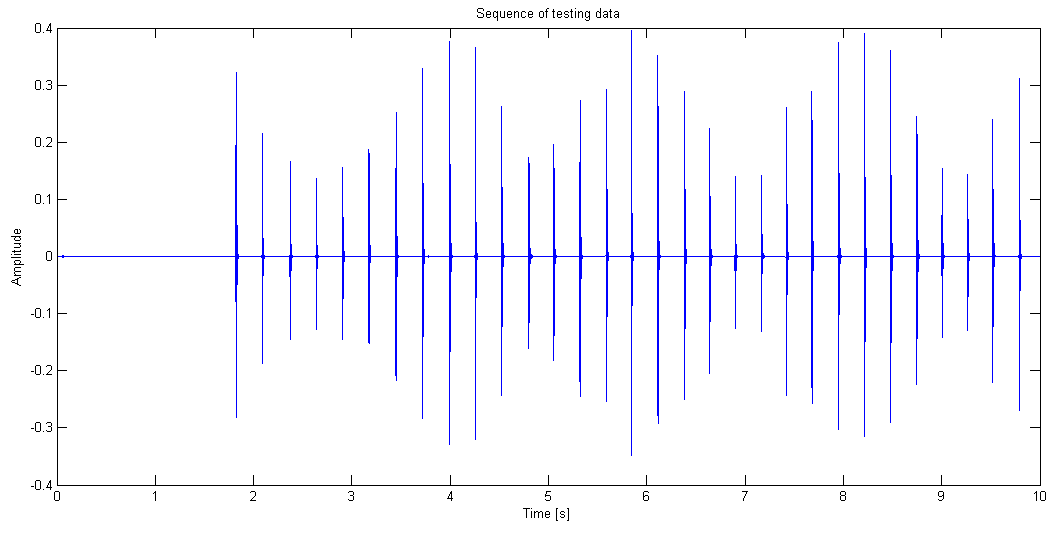
\includegraphics[width=410 px]{dataSequence.png}
\caption{Example of testing data variability.}\label{fig:dataSequence}
\end{figure}

Figure~\ref{fig:dataSequence} shows an example of a testing data sequence. While recording the testing, as well as training, data great care is taken to vary a range of parameters of the tap. From Figure~\ref{fig:dataSequence} is the clearly seen that the tapping force is varied resulting in a varying pulse amplitude, but the strike angle is also varied to replicate natural variability. The exact tapping location will also inadvertently vary due to the manual nature of the data collection.


As well as evaluating the classification performance of some of the algorithms presented above, the effect of varying various parameters of the models, such as component number and template length, is also explored.

\subsection{Amplitude variable model}
The amplitude variable PCA, henceforth known as K-PCA, model presented in section~\ref{sec:KamplitudeModel} will be compared to the standard \gls{pca}  approach from section~\ref{sec:APRpca} to gauge if there is an advantage gained by adding the additional $K$ scaling factor to the model.

The data used for this comparison will be the same as that outlined in section~\ref{sec:MultiAPRMethod} and comprises a 9 spot model trained on a wooden board. The two methods will be compared based on three different data channels/microphones each at different locations and in two different environments. Figure~\ref{fig:NoisyMicSignalsCompare} shows an example of the audio waveform for the two different environments, for two of the three channels. A total of 79 audio segments from the relatively noiseless environment and 48 from the noisy environment were used. Each segment contained a single pulse from a random spot on the surface. Details of the system can be found in appendix~\ref{ap:MultiAPRsystem}.

The templates used in the comparison were identical in all other aspects than the parameters $K$ and $p(K)$. For the varying number of scale levels $L$ numbers were chosen so that $K$ and $p(K)$ could simply be decimated and $p(K)$ re-scaled.

For each method, and for each environment, an average of the performance of the three channels/microphones is presented. The raw data for all channels can be found in appendix~\ref{ap:KPCAresults}. The K-PCA was tested with a variety of discrete scaling parameters $L$ from 1 to 100.

\section{Results}\label{sec:results}
\subsection{ML, MAP and PCA methods}
In this section the empirical evaluations of the methods mentioned above are presented.

Figure~\ref{fig:PCAperform} shows the performance of the \gls{pca} type algorithm using the training data $D^1_S$ and the testing data $D^2_S$. The figure gives an idea of how the performance changes with the changing number of components, $q$, used in the templates. Figure~\ref{fig:PCAperform} clearly shows that the rate of correct classification is beyond 90\% down to 2 components whereafter it drops off sharply to below 10 \%. It is noted that the performance drops to around 8\% which is exactly what would be expected by a random guess or the prior knowledge $p(j)= \frac{1}{J}$. A decrease in performance is detectable from 4 components and down, whereas the performance for 5 components and more appears constant.

\begin{figure}[!] %PCA components S-S
\centering
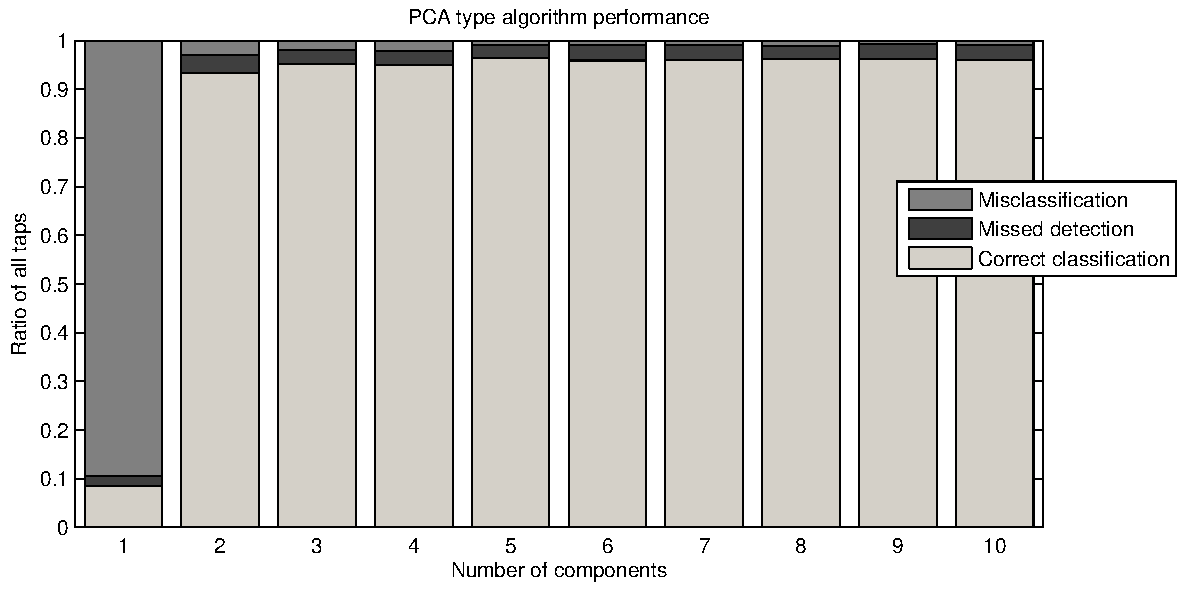
\includegraphics[width=150mm]{PCAperform.pdf}
\caption{Performance of the \gls{pca} type algorithm for different numbers of \gls{pca} components and with a template length $M=250$ samples. Training data: $D^1_S$, Testing data: $D^2_S$.}\label{fig:PCAperform}
\end{figure}

In Figure~\ref{fig:PCAperformLength} the relation between performance and template length $M$ can be seen with a test conducted with the same data as the previous test. The performance of the algorithm appears unaffected by $M$ at template lengths above 170 samples although for $M<170$ the performance decreases dramatically and as with Figure~\ref{fig:PCAperform} appears to settle around $p(j)$. The ratio between missed detections and misclassifications appear to vary greatly at low values for $M$ though it is currently not certain why this occurs. It is worth mentioning that this ratio is purely determined by a threshold in the algorithm and can be fine tuned for a desired outcome.

\begin{figure}[!] %PCA length S-S
\centering
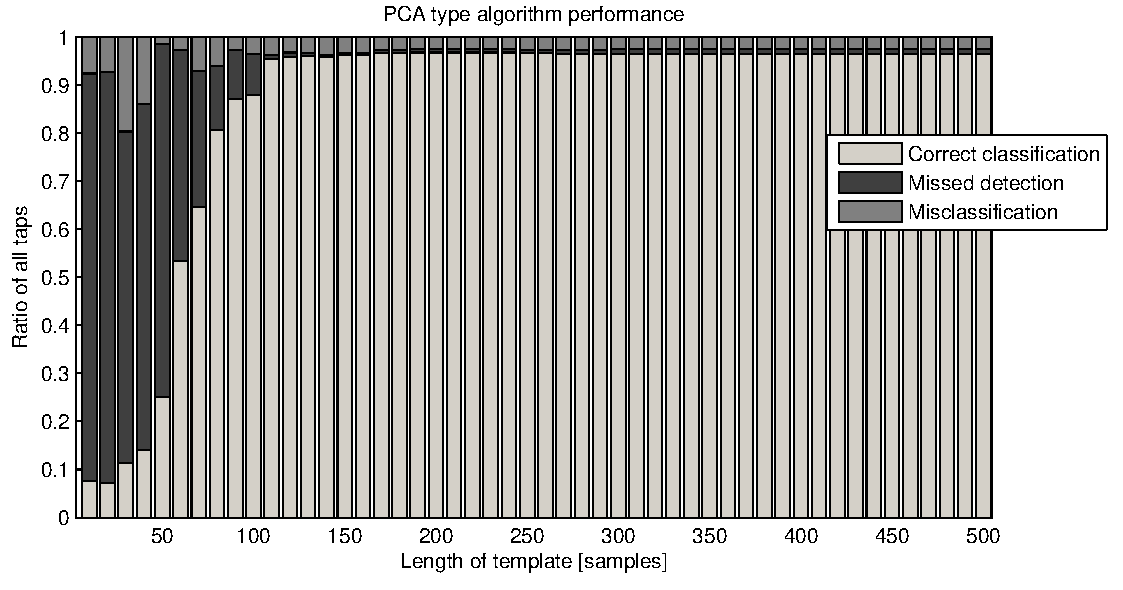
\includegraphics[width=150mm]{PCAperformLength.pdf}
\caption{Performance of the \gls{pca} type algorithm for different values of template length $M$ for components $q=5$. Training data: $D^1_S$, Testing data: $D^2_S$,}\label{fig:PCAperformLength}
\end{figure}

Figure~\ref{fig:MLperform} shows the performance of the \gls{ml} based algorithm using training data $D^1_S$ and testing data $D^2_S$. This figure shows the effect of changing the template length $M$ on the detection performance. As in Figure~\ref{fig:PCAperformLength} the performance appears to peak and stay constant at $M>170$. With the \gls{pca} algorithm the performance appears to approach the prior probability of detection at $M<50$ which, in this case, is set as being uniform across the different spots $j$.

Another feature of Figure~\ref{fig:MLperform} is the ratio of various detection results. Whereas the \gls{pca} type algorithm replaced correct classifications with misclassifications when the number of components fell below 5, the \gls{ml} algorithm appears to miss the detection of the tap entirely. This difference in the two methods is caused by a difference in the threshold for a missed detection.


\begin{figure}[!] %ML length S-S
\centering
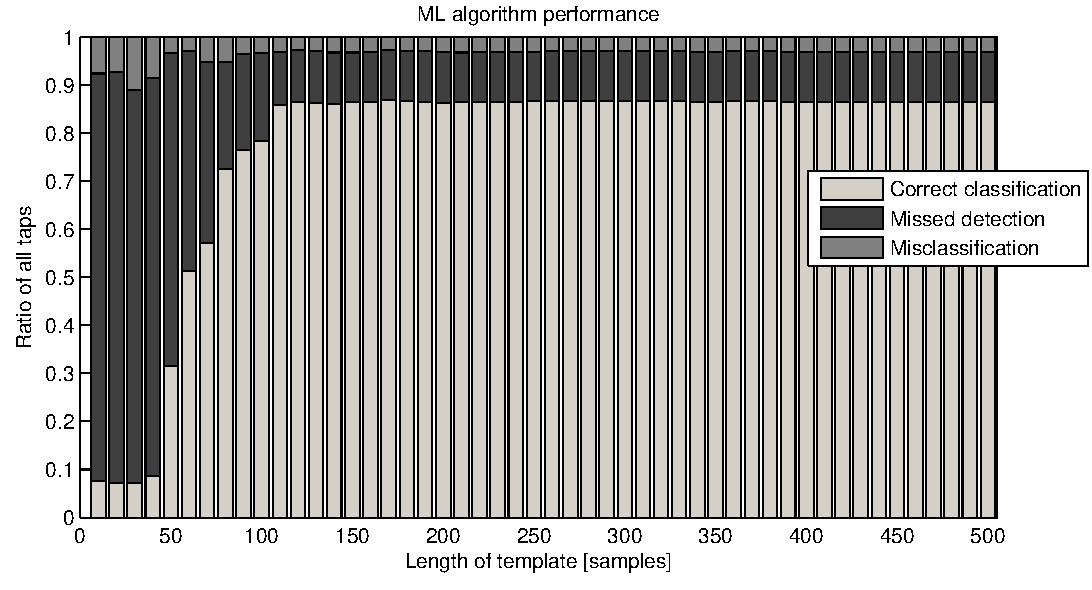
\includegraphics[width=150mm]{MLperform.pdf}
\caption{Performance of the \gls{ml} algorithm for different template sample lengths $M$. Training data: $D^1_S$, Testing data: $D^2_S$.}\label{fig:MLperform}
\end{figure}

For completeness Figure~\ref{fig:MAPperformLength} has been included to show the performance of the \gls{map} algorithm. The training and testing set up is identical to the previous evaluation of the \gls{ml} algorithm and the performance appears to be almost identical.

\begin{figure}[!] %MAP Length S-S
\centering
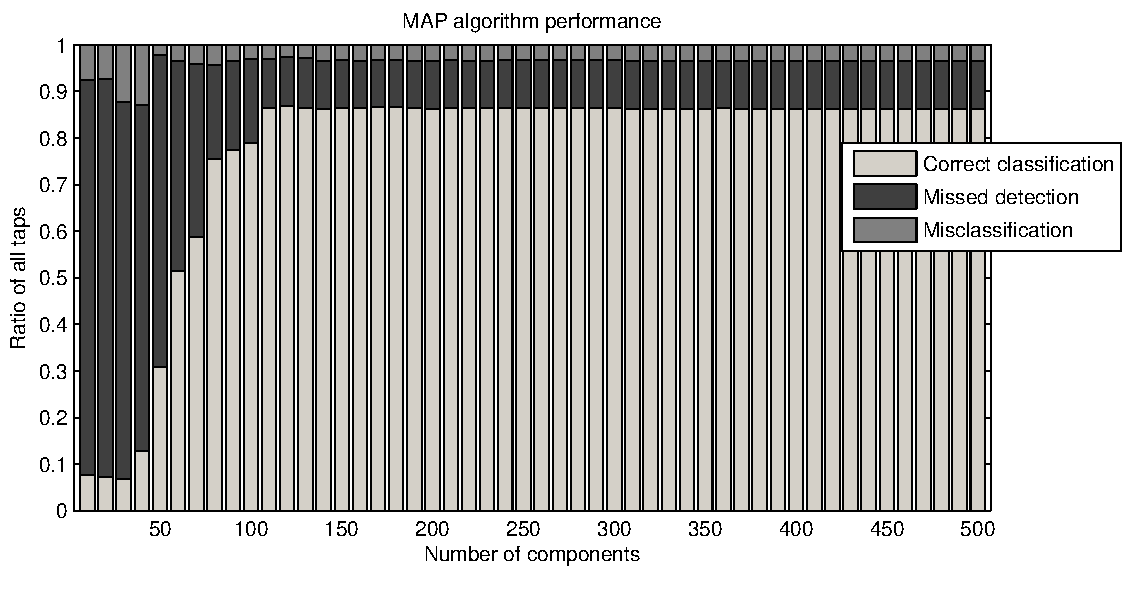
\includegraphics[width=150mm]{MAPperformLength.pdf}
\caption{Performance of the \gls{map} algorithm for different template sample lengths $M$. Training data: $D^1_S$, Testing data: $D^2_S$.}\label{fig:MAPperformLength}
\end{figure}

Figure~\ref{fig:PCAperformNail} shows the performance of the \gls{pca} type algorithm with $q$ again varying from 1 to 10, with training data $D^1_S$ and testing data $D^2_N$. In other words, the algorithm is tested by tapping using a finger nail but trained using only a stylus. This test is conducted to evaluate the \gls{pca} type algorithms ability to cope with testing data significantly different to the training data, and more specifically to evaluate the effect on the performance in relation to the number of components included, $q$. Figure~\ref{fig:PCAperformNail} shows a significantly reduced performance although the performance in relation to $q$ appears similar. For $q=1$ the performance still approaches $p(j)$.

\begin{figure}[!] %PCA components S-N
\centering
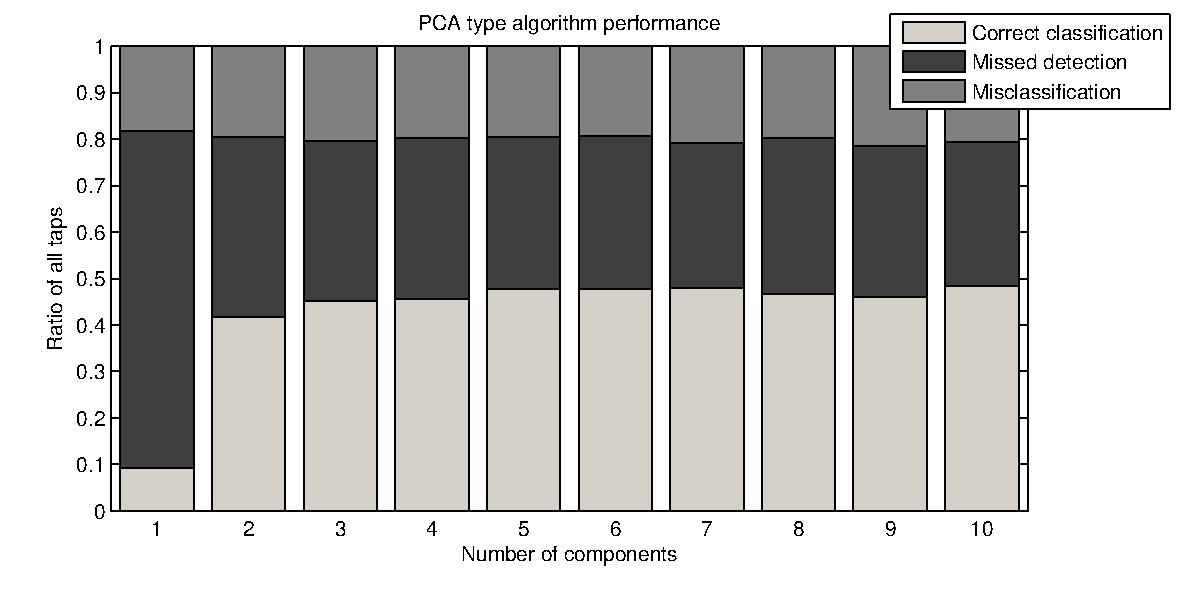
\includegraphics[width=150mm]{PCAperformNail.pdf}
\caption{Performance of the \gls{pca} type algorithm for different numbers of \gls{pca} components and with a template length of $M=250$ samples. Data used to evaluate performance was tapped using finger nails rather than the stylus used for training. Training data: $D^1_S$, Testing data: $D^2_N$.}\label{fig:PCAperformNail}
\end{figure}

The motivation for developing the \gls{pca} type algorithm was to be able to model data with a high degree of variability. Figure~\ref{fig:PCAperform_SN-SN} shows the performance of the \gls{pca} type algorithm in relation to changing $q$, with training being done with both the stylus $D^1_S$ and finger nail data $D^1_N$. By training on both sets it was hypothesised that the increased variability in the training data would be mirrored in the components, enabling the algorithm to cope with an equally increased degree of variability during the testing stage. To simulate the increased variability during the testing stage this test was conducted using stylus $D^2_S$ and finger nail $D^2_N$ data as well. Data presented in Figure~\ref{fig:PCAperform_SN-SN} suggests that this is the case.

\begin{figure}[!] %PCA components SN-SN
\centering
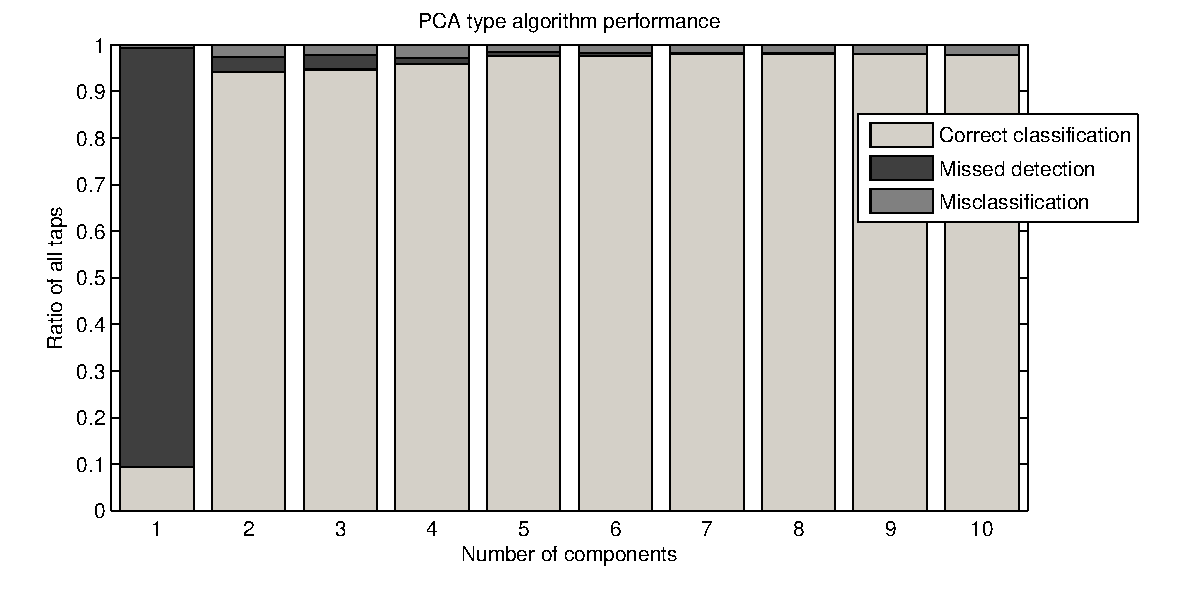
\includegraphics[width=150mm]{PCAperform_SN-SN.pdf}
\caption{Performance of the \gls{pca} type algorithm for different numbers of \gls{pca} components and with a template length $M=250$ samples. Training data: $D^1_S$ and $D^1_N$, Testing data: $D^2_S$ and $D^2_N$}\label{fig:PCAperform_SN-SN}
\end{figure}

Figure~\ref{fig:PCAMLMAPperform} gives an overview of the performance of the different algorithms with various data sets being used for testing and training. The specific data used for each test is noted on the figure itself. Please note that for all tests in Figure~\ref{fig:PCAMLMAPperform}, $M=250$ and $q=5$. These values were determined as sufficient in the previous tests detailed above.

\begin{table}\begin{center}
\caption{Classification percentage correct results per channel for each algorithm with combined stylus and nail training and testing data.}
\label{tab:APRresultsPerChan}
\begin{tabular}{|c|c|c|c|c|c|c|c|c|c|c|c|c|}\hline
  & \multicolumn{12}{|c|}{Spot} \\
\hline
Method  & 1   & 2     & 3    & 4     & 5    & 6     & 7     & 8      & 9     & 10    & 11    & 12   \\ \hline
ML      & 86  & 100   & 90   & 98    & 99   & 100   & 43    & 100    & 100   & 39    & 100   & 76   \\
MAP     & 84  & 100   & 92   & 99    & 99   & 100   & 48    & 100    & 100   & 38    & 100   & 77   \\
PCA     & 99  & 100   & 93   & 100   & 99   & 100   & 99    & 100    & 100   & 100   & 100   & 100   \\ \hline
\end{tabular}\end{center}\end{table}

Table~\ref{tab:APRresultsPerChan} shows the percentage of correct detection, based on all detections, per spot for the three different methods. This data is generated from the templates trained on both the stylus and nail tapping data and tested on both data sets as well. It is seen that on spots 2, 5, 6, 8, 9 and 11 all methods perform similarly. On spots 1, 3, 4, 7, 10 and 12 the ML and MAP methods are performing worse than the PCA. Particularly spots 7 and 10 show a significantly reduced performance in the mixed training and testing scenarios. For more spot specific results with the PCA approach Tables~\ref{tab:multiAPRresultsPerChan} and \ref{tab:multiAPRresultsNoisePerChan} should be considered.

\begin{figure}[!] %PCA-ML-MAP compare
\centering
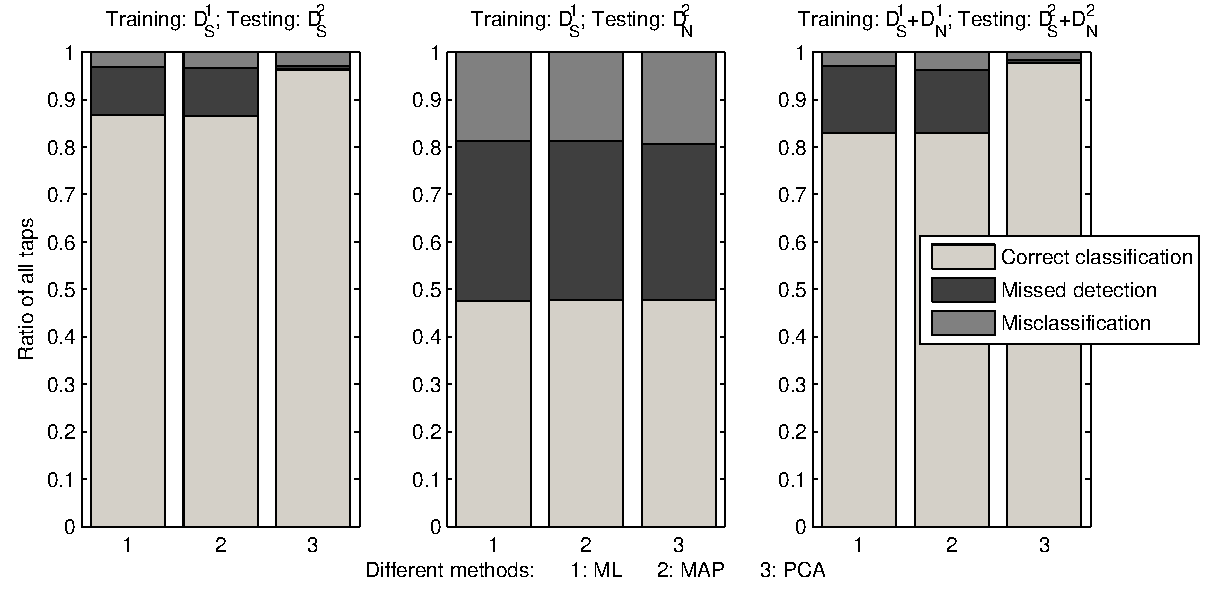
\includegraphics[width=150mm]{PCAMLMAPperform.pdf}
\caption{Performance of all 3 algorithms in 3 different tests. All tests conducted with $M=250$ and $q=5$. $D^1_S + D^1_N$ refers to two sets of data being merged together, not added.}\label{fig:PCAMLMAPperform}
\begin{picture}(0,0)
\put(-200,260){a)}
\put(-74,260){b)}
\put(55,260){c)}
\end{picture}
\end{figure}

\subsection{Sparse training extension}

A selected run of the sparse training extension, for the \gls{ml} algorithm, has given the result presented in Figure~\ref{fig:padPlot}. The intensity map shows the highest probability near the spot actually tapped, which is between spot 7 and 8. Figure~\ref{fig:padPlot} also reveals other areas of high probability. It is stressed that this run is a selected run of the algorithm and the performance is not consistently of this standard, although Figure~\ref{fig:padPlot} does provide a good representation of the algorithm when it is working, with several areas of high probability being a common feature.

\begin{figure}[!]
\centering
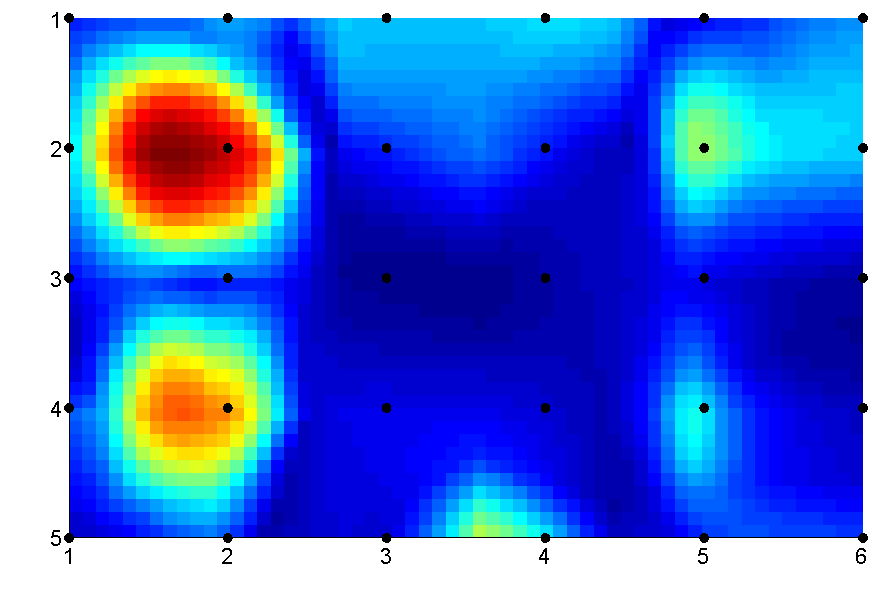
\includegraphics[width=150mm]{padPlot.pdf}
\caption{Intensity map of model probabilities. Black dots represent trained tapping spots, as seen on Figure~\ref{fig:Pad}. }\label{fig:padPlot}
\end{figure}

\subsection{Variable amplitude PCA model (K-PCA)}

The results from a comparison between the standard \gls{pca} and the K-PCA classification algorithms are presented in Figure~\ref{fig:performanceCompareKPCAPCA.pdf}. Figure~\ref{fig:performanceCompareKPCAPCA.pdf}(a) and (b) show the results from testing clean data and the noisy data respectively. For the 9 spot model, see experimental setup in Figure~\ref{fig:MultiAPRsystem.pdf}, the random chance result is shown as a dashed line well below all performance results. The performance of K-PCA appear less affected by the noisy environment than the standard approach with a mean decrease in accuracy of about 3 percentage points (pp) as opposed to a decrease of 6 pp for the standard \gls{pca} approach. A complete list of results used in Figure~\ref{fig:performanceCompareKPCAPCA.pdf} can be found in appendix~\ref{ap:KPCAresults}.

\begin{figure} %performanceCompareKPCAPCA.pdf
\begin{minipage}[b]{1.0\linewidth}
  \centering
  \centerline{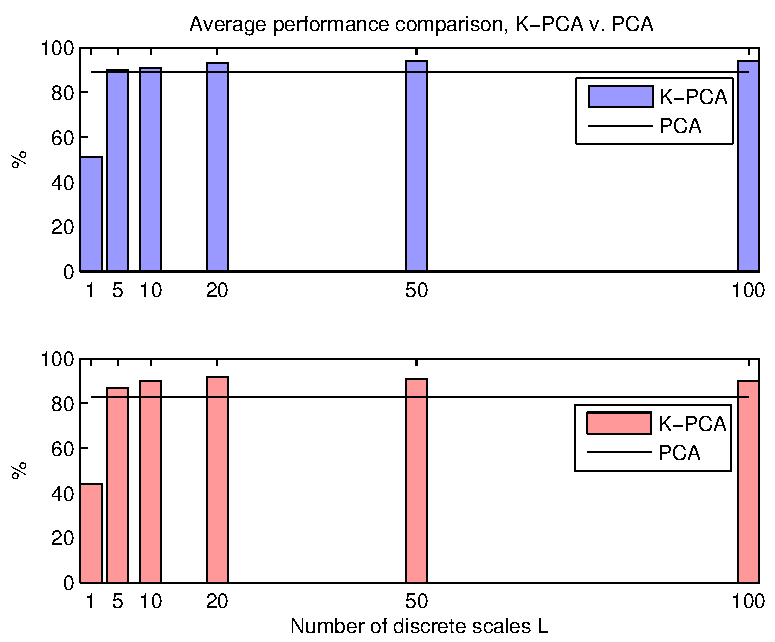
\includegraphics[width=13cm]{performanceCompareKPCAPCA.pdf}
  \begin{picture}(0,0)
\put(-335,295){(a)}
\put(-335,145){(b)}
\end{picture}}
\end{minipage}
\caption{Comparison of \gls{pca} and K-PCA (variable amplitude \gls{pca} model) methods with varying discrete scaling values $L$. (a) on clean data, (b) on noisy data.)}\label{fig:performanceCompareKPCAPCA.pdf}
\end{figure}

Computationally the case for $L=1$ should be identical to that of the standard \gls{pca} approach although Figure~\ref{fig:performanceCompareKPCAPCA.pdf} clearly shows a significant performance drop for this case. To maintain consistent performance only one set of templates were trained for this experiment and that included the case for $L=100$. The additional results gathered for lower number of scales $L$ are achieved by decimating the vector containing the values for the $p(K^j)$ and normalizing. At $L=1$ only one scaling value was chosen from $p(K^j)$ and while it was chosen in a similar fashion to the other trials of varying $L$ for $L=1$ this was the initial and lowest scale resulting in poor performance. This dip in performance should only be considered a feature of the consistent testing system and in practice K-PCA for $L=1$ should be considered identical to the standard PCA.

\section{Discussion}

The results from the previous section enable a range of assertions to be made about the relative performance of the different algorithms in various conditions. It is, for example, noticed in Figures~\ref{fig:PCAperform}, \ref{fig:PCAperformNail} and \ref{fig:PCAMLMAPperform} that the performance of the \gls{pca} varies greatly by including 2 rather than 1 components in the template set. It is also noted from Figure~\ref{fig:PCAperform} and \ref{fig:MLperform} that with only 2 components, $q=2$, the \gls{pca} easily outperforms the \gls{ml} (and MAP) method but with only 1 component, $q=1$, the performance of the \gls{pca} drops to $p(j)$. Although both the \gls{ml} and \gls{pca} are equivalent from the viewpoint of the detection for $q=1$, it is clear that their performance is not. In the case of $q=1$ what separates the two algorithms is how the template $t$ is derived. It appears that the mean template is more effective in classifying pulses than the PC is. The most likely explanation for this behavior is that the PC of one of the taps is a sufficiently broad interpretation of the tap that results in a high likelihood in each case and hence ``wins'' each classification. This hypothesis is further supported by the performance for $q=1$ in Figure~\ref{fig:PCAperform_SN-SN}, where the ratio between missed detections and misclassifications is entirely different with an overwhelming number of missed detections to misclassifications. In this case, with this training data, the PC was clearly a much less likely fit to the testing data.

Figures~\ref{fig:PCAperformLength}, \ref{fig:MLperform} and \ref{fig:MAPperformLength} consistently suggest that the performance of all algorithms appear almost unaffected by template length $M$ for lengths $M\geq110$, although a slight gradient can be noticed in all plots up to $M=170$. This slight gradient may simply be due to the trimming of the aligned taps for one of the templates. The change of template length $M$ also appears to affect all methods in a similar manner.

The \gls{pca} type algorithm was derived with the intention of creating a model being able to cope with a higher degree of variability than the \gls{ml} and \gls{map} methods. Although Figure~\ref{fig:PCAperformNail} shows relatively poor performance for different testing data to training data, it is worth noting that when the algorithm was allowed to train with data of higher variability, see Figure~\ref{fig:PCAperform_SN-SN}, a dramatic improvement was seen. This performance boost appears to even outperform the \gls{pca} with no merged data, see Figure~\ref{fig:PCAperform}, which might be explained by the increased training data which allows the derived components to be more robust to even minor variability that could potentially ``confuse'' the PCA.

Figure~\ref{fig:PCAMLMAPperform} gives a definitive insight into the relative performance between all the algorithms in various conditions, and it is clear that the \gls{pca} algorithm has a significant performance edge, specifically when it comes to testing data with greater variability. Comparing graph a and c in Figure~\ref{fig:PCAMLMAPperform} it can be seen that the greater variability in the testing data affects the methods that use a mean template negatively. The increased variability results in mean templates that focus on some broader aspects of the data and more subtle variations are lost. It is again noticed that the \gls{pca} method performs better under these circumstances.

Although no quantifiable results of the performance of the interpolated training algorithm exist, preliminary tests show that the system is able to detect some off- grid points with relative success in certain very specific regions of the board, but for the most part the results are fairly random. It is thought that this is due to problems with either alignment or more erratic and unpredictable pulses arising from certain regions. The common feature of multiple high probability regions observed in Figure~\ref{fig:padPlot} is more than likely due to symmetry in the mechanical structure being reflected in the vibrational characteristics of the device. The issue of the structural symmetry is thought to be an issue specifically on the wooden board due to its mechanical uniformity. The intensity map does generally show the correct tapping position with higher probabilities than the other peaks created by symmetry.

The proposed variable amplitude modification to the \gls{pca} algorithm (K-PCA) is shown in Figure~\ref{fig:performanceCompareKPCAPCA.pdf} to outperform the standard \gls{pca} approach and is consistently more resilient to the noisy environment. The results also showed that while the method performed significantly worse than \gls{pca} with a single amplitude scale ($L=1$) the classification performance overtook \gls{pca} by $L=5$. Above $L=20$ no discernable performance increase was noted. While no formal results are presented, during testing the K-PCA method was computationally intensive in relation to the \gls{pca} method. Preliminary profiling suggests that this was due to linear factors associated with the number of scales $L$ making the K-PCA algorithm with $L=20$ approximately 20 times slower. For the other approaches tested the computational times were all comparable.

\section{Conclusions}
%rewriten
From the results presented in this chapter it is clear that it is possible to implement an \gls{apr} system using a single input channel. All algorithms proposed outperformed random chance by a margin and gave false classifications in less than 10\% of the tests in ideal situations. For tangible primary interface technology a classification rate of 100\% or near 100\% is required in addition to higher active spot resolution and stronger resilience to environmental and tapping types. While the requirements for a direct touch-screen replacement might be out of reach for this current implementation, it is possible to either let the technology serve as an off-the-screen touch augmentation, or perhaps in classification applications on recorded data where post-hoc training is possible.

%difficult situations
Despite reduced correct classification rates on highly variable testing and training data for the case of the \gls{map} and \gls{ml} algorithms, Figures~\ref{fig:PCAMLMAPperform}(a) and (c) showed that the \gls{pca} algorithm increased its performance with a larger training and testing basis as hypothesised. For the unfamiliar testing data in Figure~\ref{fig:PCAMLMAPperform}(b) the \gls{pca} algorithm performed similarly to the other algorithms.

For a large number of models $J$ a manual training task quickly becomes laborious and a high resolution touch interface, similar to current touchscreen technologies, requires the implementation of the sparse training extension. Early results show that some interpolation between discrete points is possible but due to the homogeneous nature of the surface used, competing feasible classes may have been more numerous than with a less homogeneous material. This could increase the difficulty of interpolation between spots for the \gls{ml} and \gls{map} approaches.

Computational constraints on implementation of multiple models/spots $J$ or amplitude scales $L$ in the case of K-PCA could in part be mitigated by computational optimisation realising that all added complexity is parallelisable.

\subsection{Possible future work}
% Better PCA component choices
% Improve and extend Sparse Training to PCA
\subsubsection{Sparse Training applied to PCA and common PCA components}
The preliminary study of the sparse training extension showed that this approach is possible with even the simplest interpolation approaches. A study into the extent to which individual components in the \gls{pca} approach vary over a surface could lead to a straight forward \gls{pca} implementation of the sparse training approach. While this first approach assumes that equivalent components are identifiable at neighbouring active spots, it might be easier to achieve this goal by drawing the random components from an ensemble of the entire training set data (i.e. from all models) and then identifying their contribution in each model. This would have the additional advantage of compressing the training data needed and possibly also provide a different approach to filtering out non-essential components for classification.

% Focus more of the additional work on the K-PCA method and evaluate missed detections and general sensitivity.
\subsubsection{Additional K-PCA evaluation}
While the \gls{pca} algorithm represents the best approach that was extensively tested in this chapter, the K-PCA did outperform \gls{pca} on pure classification performance. While the underlying K-PCA model does, at least theoretically, model pulses of varying amplitudes, it is also possible that this added flexibility increased the model's response to other kinds of noise. Further studies should focus on comparing the two algorithms' general sensitivity to establish a margin between correct and false detections. Given dedicated detection algorithms proposed here, and later in this work, this specific margin might not be of ultimate importance.

% Perform tonal pre processing
\subsubsection{Separation pre-processing stage}
Figure~\ref{fig:performanceCompareKPCAPCA.pdf} provided a clear indication that the noisy environment made the classification scenario more difficult. In light of this it is possible that the separation pre-processing stage developed in section~\ref{sec:WPseparation} could provide improved resilience to music and speech which is well modeled in this fashion. Removing spurious tonal components may even increase classification performance by removing more general standing waves within the device in question.
% ------------------------------------------------------------------------


%%% Local Variables:
%%% mode: latex
%%% TeX-master: "../thesis"
%%% End:
